\documentclass[11pt]{article}
\usepackage[margin=1.05in]{geometry}
\usepackage[T1]{fontenc}
\usepackage{lmodern}
\usepackage{microtype}
\usepackage{amsmath,amssymb,amsthm,mathtools}
\usepackage{enumitem}
\usepackage{xcolor}
\usepackage{hyperref}
\usepackage[nameinlink,noabbrev]{cleveref}
\usepackage{tikz}
\usetikzlibrary{calc}
\usepackage{booktabs}

\hypersetup{
  colorlinks=true,
  linkcolor=blue!45!black,
  citecolor=blue!45!black,
  urlcolor=blue!45!black,
  pdftitle={Extended Parallel Bodies and a Steiner Formula for Planar PL Sets}
}

\newtheorem{theorem}{Theorem}[section]
\newtheorem{lemma}[theorem]{Lemma}
\newtheorem{proposition}[theorem]{Proposition}
\newtheorem{corollary}[theorem]{Corollary}
\newtheorem{definition}[theorem]{Definition}
\newtheorem{remark}[theorem]{Remark}

\crefname{theorem}{theorem}{theorems}
\crefname{lemma}{lemma}{lemmas}
\crefname{proposition}{proposition}{propositions}
\crefname{corollary}{corollary}{corollaries}
\crefname{definition}{definition}{definitions}
\crefname{remark}{remark}{remarks}

\newcommand{\R}{\mathbb R}
\newcommand{\Area}{\operatorname{Area}}
\newcommand{\Vol}{\operatorname{Vol}}
\newcommand{\len}{\operatorname{len}}
\newcommand{\dist}{\operatorname{dist}}
\newcommand{\relint}{\operatorname{relint}}
\newcommand{\Edges}{\operatorname{Edges}}
\newcommand{\Vertices}{\operatorname{Vertices}}
\newcommand{\AH}{\operatorname{AH}}
\newcommand{\AHcon}{\operatorname{AH}_{\mathrm{con}}}
\newcommand{\AHext}{\operatorname{AH}_{\mathrm{ext}}}
\newcommand{\AHfar}{\operatorname{AH}_{\mathrm{far}}}
\newcommand{\AHnear}{\operatorname{AH}_{\mathrm{near}}}
\newcommand{\Steiner}{\mathbf S}
\newcommand{\calE}{\mathcal E}
\newcommand{\eps}{\varepsilon}
\newcommand{\closedball}[2]{B_{#2}(#1)}
\newcommand{\openball}[2]{B_{#2}^{\circ}(#1)}
\newcommand{\sq}{\mathbin{\sqcup}}

\DeclareMathOperator{\conv}{conv}

\setlist[itemize]{topsep=4pt,itemsep=2pt}
\setlist[enumerate]{topsep=4pt,itemsep=2pt}

\numberwithin{equation}{section}
 
\title{Extended Parallel Bodies and a Steiner Formula for Planar PL Sets}
\author{Joseph T. Previdi}
\date{\today}

\begin{document}
\maketitle

\begin{abstract}In this paper, given an arbitrary piecewise-linear (PL) set $A$ in the plane, we give an elementary geometric construction for a physical region whose area precisely equals the Steiner polynomial $\mathbf{S}(A,r)$ evaluated at small $r$. Specifically, for a set $A\subset\R^2$ and $r\ge 0$, we define its \textit{extended $r$-parallel body} $E(A,r)$ as precisely those points $x$ such that every closed radius-$r$ ball containing $x$ intersects the ordinary parallel body $A_r$. For a closed planar PL set $A$, we prove that for all sufficiently small $r>0$,
	\[
	\Area(E(A,r))=\mathbf{S}(A,r)=\Area(A)+2\mu_1(A)r+\pi\chi(A)r^2,
	\]
	where $\mu_1$ is the first intrinsic volume and $\chi$ is the Euler characteristic. 
	
	$E(A,r)$ may be characterized as the $r$-erosion of the $2r$-parallel body. For closed convex sets, this is precisely the $r$-parallel body. We give an explicit admissible radius for the above identity. This identity is established by explicitly constructing $E(A,r)$ by appending geometric "arrowhead" shapes to $A_r$. The argument proceeds by inductively deleting simplices from the convex hull of $A$ and tabulating corresponding deletion or addition of arrowheads. The main theorem and its geometric proof are formalized in Lean 4, relative only to the classical planar Steiner formulas.
	
	For non-closed PL sets, we demonstrate that the Steiner polynomial still represents the area of a geometrically defined region obtained from the extended parallel bodies of its successive missing frontiers. In fact, we prove that under certain conditions a set-valued construction (such as $E$) on closed sets whose volume realizes a valuation must induce a corresponding physical realization for non-closed sets. 
	
	The planar PL result therefore provides one example in which a valuation polynomial is realized as the Lebesgue measure of a specific region near the original set, even in the presence of singularities where ordinary parallel bodies fail to admit such a formula. This suggests it may be possible to similarly manifest the Steiner polynomial in higher dimensions or non-PL cases.
\end{abstract}

\tableofcontents

\section{Introduction}

For a compact convex set $K\subset\R^2$, the classical Steiner formula expresses the area of its ordinary parallel body as
\[
\Area(K_r)=\Area(K)+2\mu_1(K)r+\pi r^2,
\]
where $\mu_1(K)$ is the first intrinsic volume; for a convex polygon, $2\mu_1(K)$ is its perimeter. This polynomial behavior is one of the basic manifestations of curvature and intrinsic-volume theory. Extensions to sets of positive reach and local parallel-volume formulas for much more general closed sets are classical subjects; see, for example, Federer~\cite{Federer1959}, Schneider~\cite{Schneider2014}, and Hug--Last--Weil~\cite{HugLastWeil2004}.

The present paper studies a different geometric object. Given a set $A\subset\R^n$ and a scale $r\ge0$, define $E(A,r)$ by requiring that every closed radius-$r$ ball containing a point $x$ meet the ordinary $r$-parallel body $A_r$. This definition is elementary and dimension-independent. A first observation is that
\[
E(A,r)=\{x:B_r(x)\subseteq A_{2r}\},
\]
so $E(A,r)$ is the erosion of $A_{2r}$ by a radius-$r$ ball. For convex sets this operation agrees with the ordinary parallel body, but for singular sets it may add regions outside $A_r$.

Our main result identifies those added regions explicitly for finite planar PL sets and proves that their total area restores the planar Steiner polynomial.

\begin{theorem}[Planar PL extended Steiner formula]\label{thm:main-intro}
Let $A\subset\R^2$ be a nonempty closed PL set. Then there exists $R>0$ such that for every $0<r<R$,
\[
\boxed{
\Area(E(A,r))
=
\Steiner(A,r)
:=
\Area(A)+2\mu_1(A)r+\pi\chi(A)r^2.
}
\]
Moreover, $R$ may be chosen explicitly from any finite triangulation of $\conv(A)$ refining a simplicial representation of $A$; see \cref{def:MR}.
\end{theorem}

The proof has two main components. First, for small $r$ we characterize $E(A,r)$ as the disjoint union of $A_r$ with finitely many explicit \emph{exterior consecutive arrowheads} associated to pairs of incident edges. Second, we triangulate the convex hull of $A$ and remove the relatively open simplices not belonging to $A$, in descending dimension. The change in $\Area(E(\cdot,r))$ caused by deleting each open simplex is shown to equal its Steiner valuation. The deletion of an isolated open edge is the technical core; its proof is a local cancellation between ordinary offset overlap and the creation or deletion of arrowheads.

Although the main theorem is stated for closed PL sets, closedness is not essential to the final formulation. Once a closed-set identity
\[
\Vol_n(E(C,r))=\Steiner(C,r)
\]
is known on a class stable under closure and missing frontiers, an abstract finite frontier filtration gives an alternating physical region whose ordinary volume is $\Steiner(A,r)$ for nonclosed $A$. In the planar PL case this yields
\[
\Area\Bigl([A^r\setminus F(A)^r]\sqcup F^2(A)^r\Bigr)
=
\Steiner(A,r),
\qquad A^r:=E(A,r),
\]
where $F(A)=\overline A\setminus A$.

The paper is organized as follows. \Cref{sec:prelim} develops the extended parallel body and fixes the global PL separation scale. \Cref{sec:arrowheads} introduces the arrowhead geometry. \Cref{sec:characterization} proves the consecutive-arrowhead characterization of $E(A,r)$. \Cref{sec:edge-deletion} proves the isolated-edge deletion formula. \Cref{sec:main-proof} completes the main theorem by simplex deletion, and \cref{sec:frontier} gives the abstract extension to nonclosed sets.
 \section{Preliminaries}\label{sec:prelim}

\subsection{PL sets, parallel bodies, and the Steiner valuation}

For a set $A\subset\R^n$ and $r\ge0$, its closed $r$-parallel body is
\[
A_r:=\{x\in\R^n:d(x,A)\le r\}.
\]
Since $d(x,A)=d(x,\overline A)$, one always has $A_r=(\overline A)_r$.

\begin{definition}[PL set]\label{def:pl-set}
A set $A\subset\R^n$ is \emph{piecewise linear} (PL) if it is the union of finitely many relative interiors of simplices of a finite simplicial complex. A closed PL set is therefore the underlying set of a finite subcomplex after passing to a common refinement.
\end{definition}

On planar polyhedral sets we use the finitely additive intrinsic-volume valuations $\mu_1$ and $\chi$, with $\chi$ the compactly supported (equivalently, o-minimal) Euler characteristic. For compact sets, $\chi$ agrees with the usual Euler characteristic. We write
\begin{equation}\label{eq:steiner-polynomial}
\Steiner(A,r):=\Area(A)+2\mu_1(A)r+\pi\chi(A)r^2.
\end{equation}
For a compact convex polygon, $2\mu_1$ is its perimeter and $\chi=1$.

We shall repeatedly use the values of \eqref{eq:steiner-polynomial} on relatively open simplices. If $D$ is an open triangle of area $a$ and perimeter $p$, an open segment of length $L$, or a point, respectively, then finite additivity gives
\begin{align}
\Steiner(D,r)&=a-pr+\pi r^2, \label{eq:S-open-triangle}\\
\Steiner(D,r)&=2Lr-\pi r^2, \label{eq:S-open-edge}\\
\Steiner(D,r)&=\pi r^2. \label{eq:S-point}
\end{align}
Indeed, $\chi$ takes the values $1,-1,1$ on relatively open simplices of dimensions $2,1,0$, respectively; $\mu_1$ equals $-p/2$ on an open triangle, $L$ on an open segment, and $0$ on a point.

\subsection{The extended parallel body}

\begin{definition}[Extended parallel body]\label{def:extended-parallel}
For a set $A\subset\R^n$ and $r\ge0$, the \emph{extended $r$-parallel body} $E(A,r)$ is the set of all points $x\in\R^n$ for which every closed radius-$r$ ball $B_r\ni x$ has nonempty intersection with $A_r$.
\end{definition}

The following elementary reformulation is fundamental.

\begin{theorem}[Characterization of the extended parallel body]\label{thm:erosion-characterization}
For every $A\subset\R^n$ and every $r\ge0$,
\[
\boxed{
E(A,r)=\{x\in\R^n:B_r(x)\subseteq A_{2r}\}.
}
\]
Equivalently,
\[
E(A,r)=A_{2r}\ominus B_r,
\]
where $\ominus$ denotes morphological erosion by the closed radius-$r$ ball. In particular,
\[
A_r\subseteq E(A,r)\subseteq A_{2r}.
\]
\end{theorem}

\begin{proof}
We first show that for every $z\in\R^n$,
\begin{equation}\label{eq:ball-meets-offset-iff}
B_r(z)\cap A_r\ne\varnothing
\quad\Longleftrightarrow\quad
z\in A_{2r}.
\end{equation}
If $y\in B_r(z)\cap A_r$, then
\[
d(z,A)\le d(z,y)+d(y,A)\le2r.
\]
Conversely, if $z\in A_{2r}$, choose $a\in\overline A$ with $d(z,a)=d(z,A)\le2r$ and put $m=(z+a)/2$. Then
\[
d(z,m)\le r,
\qquad
d(m,A)=d(m,\overline A)\le d(m,a)\le r,
\]
so $m\in B_r(z)\cap A_r$.

Now $x\in E(A,r)$ if and only if $B_r(z)\cap A_r\ne\varnothing$ for every center $z$ such that $x\in B_r(z)$. Since
\[
x\in B_r(z)\quad\Longleftrightarrow\quad z\in B_r(x),
\]
\eqref{eq:ball-meets-offset-iff} gives
\[
\begin{aligned}
x\in E(A,r)
&\Longleftrightarrow z\in A_{2r}\quad\text{for every }z\in B_r(x)\\
&\Longleftrightarrow B_r(x)\subseteq A_{2r}.
\end{aligned}
\]
The inclusion $E(A,r)\subseteq A_{2r}$ follows because $x\in B_r(x)$, while $A_r\subseteq E(A,r)$ follows directly from the definition.
\end{proof}


\begin{figure}[htbp]
\centering
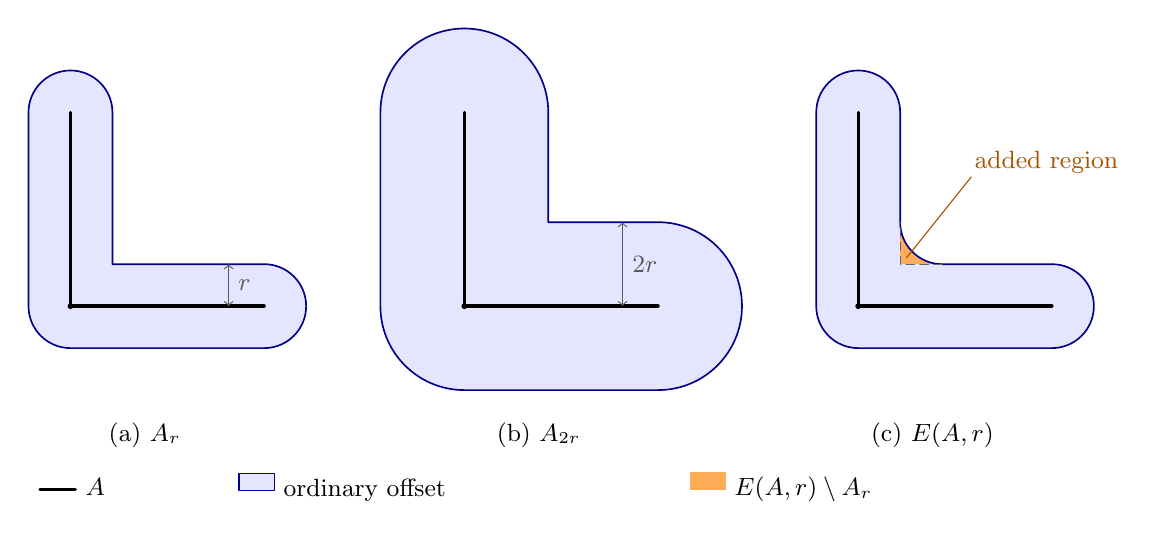
\begin{tikzpicture}[scale=0.82,line join=round,line cap=round,
  every node/.style={font=\small}]
  % Exact offsets of two perpendicular segments of length L, with r=0.65.
  \def\rad{0.65}
  \def\ell{3.0}
  \newcommand{\offsetpath}[1]{%
    (0,-#1)--(\ell,-#1) arc[start angle=-90,end angle=90,radius=#1]
    --(#1,#1)--(#1,\ell) arc[start angle=0,end angle=180,radius=#1]
    --(-#1,0) arc[start angle=180,end angle=270,radius=#1]--cycle}
  \newcommand{\originalL}{%
    \draw[black,very thick] (\ell,0)--(0,0)--(0,\ell);
    \fill (0,0) circle[radius=1.3pt];}
  \begin{scope}[xshift=0cm]
    \filldraw[fill=blue!10,draw=blue!55!black,semithick] \offsetpath{\rad};
    \originalL
    \draw[<->,black!65,thin] (2.45,0)--(2.45,\rad)
      node[midway,right] {$r$};
    \node[anchor=north] at (1.15,-1.65) {(a) $A_r$};
  \end{scope}
  \begin{scope}[xshift=6.1cm]
    \filldraw[fill=blue!10,draw=blue!55!black,semithick] \offsetpath{1.30};
    \originalL
    \draw[<->,black!65,thin] (2.45,0)--(2.45,1.30)
      node[midway,right] {$2r$};
    \node[anchor=north] at (1.15,-1.65) {(b) $A_{2r}$};
  \end{scope}
  \begin{scope}[xshift=12.2cm]
    \fill[blue!10] \offsetpath{\rad};
    % The far arrowhead is the square corner minus the open quarter disk.
    \fill[orange!65] (\rad,\rad)--(1.30,\rad)
      arc[start angle=-90,end angle=-180,radius=\rad]--cycle;
    \draw[blue!55!black,semithick]
      (0,-\rad)--(\ell,-\rad)
      arc[start angle=-90,end angle=90,radius=\rad]
      --(1.30,\rad) arc[start angle=-90,end angle=-180,radius=\rad]
      --(\rad,\ell) arc[start angle=0,end angle=180,radius=\rad]
      --(-\rad,0) arc[start angle=180,end angle=270,radius=\rad]--cycle;
    \draw[black!60,densely dashed,thin] (1.30,\rad)--(\rad,\rad)--(\rad,1.30);
    \originalL
    \draw[orange!65!black,thin] (0.75,0.75)--(1.75,2.0)
      node[above right,inner sep=1pt] {added region};
    \node[anchor=north] at (1.15,-1.65) {(c) $E(A,r)$};
  \end{scope}
  \node[anchor=west] at (-0.65,-2.8) {\tikz[baseline=-0.55ex]\draw[very thick] (0,0)--(0.45,0);\ $A$};
  \node[anchor=west] at (2.45,-2.8) {\tikz[baseline=-0.55ex]\filldraw[fill=blue!10,draw=blue!55!black] (0,0) rectangle (0.45,0.22);\ ordinary offset};
  \node[anchor=west] at (9.45,-2.8) {\tikz[baseline=-0.55ex]\fill[orange!65] (0,0) rectangle (0.45,0.22);\ $E(A,r)\setminus A_r$};
\end{tikzpicture}
\caption{The ordinary and extended parallel bodies of two perpendicular segments meeting at a common endpoint. The erosion of $A_{2r}$ by a radius-$r$ disk retains the orange corner region in addition to $A_r$. All three panels use the same scale; here the segment lengths exceed $4r$.}
\label{fig:extended-offset-example}
\end{figure}

Two immediate structural properties will be used repeatedly.

\begin{lemma}[Closure invariance and monotonicity]\label{lem:closure-monotone}
For all sets $A,B\subset\R^n$ and all $r\ge0$,
\[
E(A,r)=E(\overline A,r),
\]
and if $A\subseteq B$, then
\[
E(A,r)\subseteq E(B,r).
\]
\end{lemma}

\begin{proof}
Closure invariance follows from $A_r=(\overline A)_r$. If $A\subseteq B$, then $A_r\subseteq B_r$, so every radius-$r$ ball meeting $A_r$ also meets $B_r$.
\end{proof}

\begin{lemma}[Balls around $2r$-boundary points]\label{lem:boundary-ball}
Let $A\subset\R^n$, let $r>0$, and let $c\in\partial A_{2r}$. Then
\[
\boxed{E(A,r)\cap B_r^\circ(c)=\varnothing.}
\]
\end{lemma}

\begin{proof}
Let $x\in B_r^\circ(c)$, and hence $c\in B_r^\circ(x)$. Since $c\in\partial A_{2r}$, the neighborhood $B_r^\circ(x)$ contains a point outside $A_{2r}$. Thus $B_r(x)\nsubseteq A_{2r}$, and \cref{thm:erosion-characterization} gives $x\notin E(A,r)$.
\end{proof}

\begin{proposition}[Convex agreement]\label{prop:convex-agreement}
If $A\subset\R^n$ is nonempty, closed, and convex, then
\[
\boxed{E(A,r)=A_r\qquad(r\ge0).}
\]
\end{proposition}

\begin{proof}
The inclusion $A_r\subseteq E(A,r)$ is general. Let $x\notin A_r$ and put $\rho=d(x,A)>r$. Let $p$ be the metric projection of $x$ onto $A$ and set $u=(x-p)/\rho$. Convexity gives
\[
\langle u,a-p\rangle\le0\qquad(a\in A).
\]
Put $q=p+ru$. Then $q\in A_r$, and the same normal-cone inequality shows that $q$ is the metric projection of $x$ onto $A_r$. Now let
\[
c=x+ru.
\]
The ray $p+tu$ remains normal to $A_r$ at $q$, so
\[
d(c,A_r)=d(c,q)=\rho>r.
\]
Since $x\in B_r(c)$ but $B_r(c)\cap A_r=\varnothing$, the defining condition for $E(A,r)$ fails at $x$.
\end{proof}

\subsection{A global PL scale}\label{subsec:global-scale}

Let $A\subset\R^2$ be a nonempty closed PL set. Choose once and for all a finite simplicial complex $K$ whose underlying set is $\conv(A)$ and which refines a simplicial representation of $A$. All PL sets appearing later in the deletion argument are unions of relative interiors of simplices of this same complex.

\begin{definition}[Separation and admissible radius]\label{def:MR}
Let
\[
M:=\min_{v\notin\sigma}d(v,\sigma),
\]
with the convention $M=+\infty$ if the indexing set is empty (the single-vertex degenerate case).
where $v$ ranges over vertices of $K$ and $\sigma$ over simplices of $K$ not having $v$ as a vertex. Let $\Psi$ be the finite set of nonzero non-reflex angles between distinct incident edges of $K$; if $\Psi=\varnothing$, set $\Psi=\{\pi\}$. Define
\[
Q:=\max_{\psi\in\Psi}\left(1+\frac12\csc\frac\psi2\right),
\qquad
\boxed{R:=\frac{M}{8Q}.}
\]
Throughout the PL part of the paper we assume
\[
0<r<R.
\]
\end{definition}

Except in the single-vertex convention above, the simplicial-complex intersection property implies that a vertex which is not a vertex of a simplex is disjoint from that simplex, so $M>0$. The definition also yields the following estimates, which will be used without further comment.

\begin{figure}[!htbp]
\centering
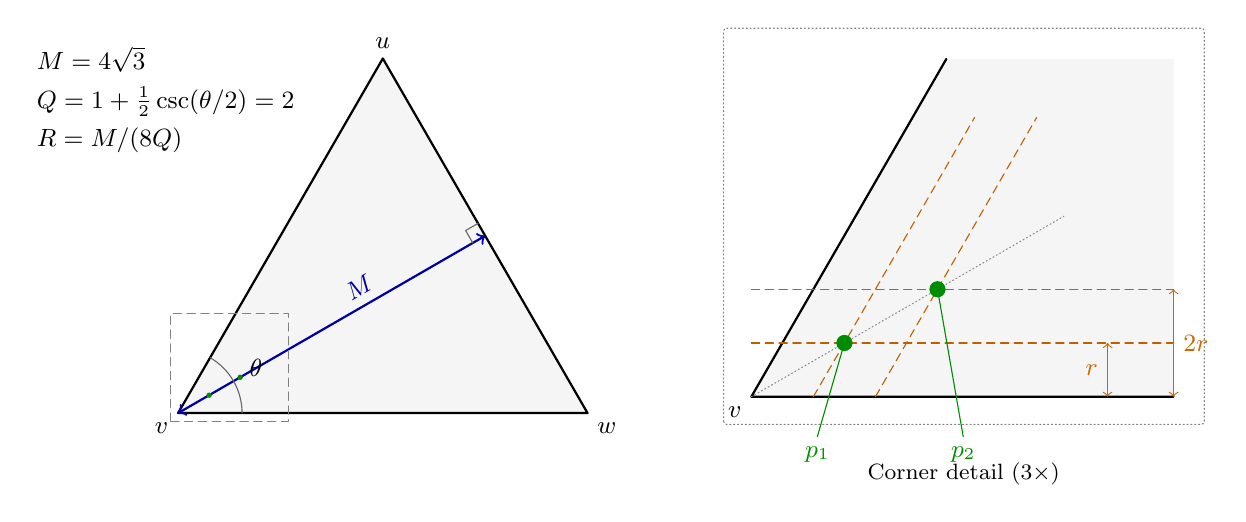
\begin{tikzpicture}[scale=0.65,line join=round,line cap=round,every node/.style={font=\small}]

  \coordinate (v) at (0,0); \coordinate (b) at (8,0); \coordinate (c) at (4,{4*sqrt(3)});
  \coordinate (m) at (6,{2*sqrt(3)});
  \filldraw[fill=black!4,thick] (v)--(b)--(c)--cycle;
  \draw[blue!65!black,thick,<->] (v)--(m) node[pos=.62,above,sloped] {$M$};
  \draw[black!60,thin] ($(m)+(-150:.28)$)--++(120:.28)--++(30:.28);
  \draw[black!60] (1.25,0) arc[start angle=0,end angle=60,radius=1.25];
  \node at (1.52,.88) {$\theta$};
  \fill[green!55!black] ({.35*sqrt(3)},.35) circle[radius=1.5pt];
  \fill[green!55!black] ({.7*sqrt(3)},.7) circle[radius=1.5pt];
  \draw[black!50,densely dashed] (-.15,-.16) rectangle (2.15,1.95);
  \node[below left] at (v) {$v$}; \node[below right] at (b) {$w$}; \node[above] at (c) {$u$};
  \node[align=left,anchor=north west] at (-2.95,7.35) {$M=4\sqrt3$\\[3pt]$Q=1+\frac12\csc(\theta/2)=2$\\[3pt]$R=M/(8Q)$};
  % Magnify the local construction without changing the admissible radius.
  \begin{scope}[shift={(11.20,.32)},scale=3.0]
    \draw[black!50,densely dotted,rounded corners=1pt] (-.18,-.18) rectangle (2.95,2.40);
    \fill[black!4] (0,0)--(2.75,0)--(2.75,2.2)--({2.2/tan(60)},2.2)--cycle;
    \draw[thick] (2.75,0)--(0,0)--(60:2.54);
    \foreach \t in {1,2}{
      \draw[orange!75!black,densely dashed] (0,{.35*\t})--(2.75,{.35*\t});
      \draw[orange!75!black,densely dashed] ({.35*\t/sin(60)},0)--++(60:2.1);
    }
    \draw[black!45,thin,densely dotted] (0,0)--(30:2.35);
    \fill[green!55!black] ({.35*sqrt(3)},.35) circle[radius=1.5pt];
    \fill[green!55!black] ({.7*sqrt(3)},.7) circle[radius=1.5pt];
    \draw[green!55!black,thin] ({.35*sqrt(3)},.35)--(.43,-.26) node[below,text=green!55!black] {$p_1$};
    \draw[green!55!black,thin] ({.7*sqrt(3)},.7)--(1.38,-.26) node[below,text=green!55!black] {$p_2$};
    \draw[orange!80!black,<->,thin] (2.32,0)--(2.32,.35) node[midway,left] {$r$};
    \draw[orange!80!black,<->,thin] (2.75,0)--(2.75,.7) node[midway,right] {$2r$};
    \node[below left] at (0,0) {$v$};
  \end{scope}
  \node[anchor=north,font=\footnotesize] at (15.35,-.78) {Corner detail ($3\times$)};

\end{tikzpicture}
\caption{Illustration of the quantities in Definition~\ref{def:MR}: in this equilateral single-triangle complex the minimum vertex--opposite-edge distance is $M$, each incident angle is $\theta=\pi/3$, $Q=2$, and $R=M/16$. The enlarged corner detail (magnification $3\times$) shows $p_1$ and $p_2$, the intersections of the inward parallels at distances $r$ and $2r$. The displayed example uses $r=0.35<R$.}
\label{fig:global-scale}
\end{figure}

\begin{lemma}[Basic separation estimates]\label{lem:basic-separation}
For every incident angle $\theta\in(0,\pi]$ occurring in $K$,
\begin{equation}\label{eq:radius-master-bound}
2r\left(1+\frac12\csc\frac\theta2\right)<\frac M4.
\end{equation}
Consequently,
\[
r\csc\frac\theta2<\frac M4,
\qquad
2r\csc\frac\theta2<\frac M2.
\]
Moreover,
\[
R\le\frac{M}{12},
\]
every edge of $K$ has length at least $M$, distinct vertices are at distance at least $M$, and disjoint simplices are at distance at least $M$.
\end{lemma}

\begin{proof}
The first estimate follows directly from $r<R$ and the definition of $Q$. Since $Q\ge 1+\tfrac12=\tfrac32$, one has $R\le M/12$. If $e=[v,w]$ is an edge, then $v$ is not a vertex of the simplex $\{w\}$, hence $\len(e)=d(v,w)\ge M$. The remaining separation statements follow similarly; for two disjoint planar simplices, a minimizing pair may be chosen with one point a vertex of one simplex.
\end{proof}
 \section{Arrowhead geometry}\label{sec:arrowheads}

Let $e_1,e_2$ be distinct incident edges of $K$ meeting at a vertex $v$, and let $\theta\in(0,\pi)$ be their non-reflex angle. Write $\widehat e_i$ for the unit vector along $e_i$ pointing away from $v$.

\subsection{The points \texorpdfstring{$p_\alpha$}{p-alpha}}

For $\alpha\in\R$, define
\begin{equation}\label{eq:palpha-def}
p_\alpha(e_1,e_2)
:=
v+\alpha r\csc\theta\,(\widehat e_1+\widehat e_2).
\end{equation}
When the angle is $\pi$, $p_\alpha(e_1,e_2)$ is left undefined; every arrowhead involving such a pair will be declared empty.

\begin{lemma}[$p_\alpha$ lemma]\label{lem:palpha}
Suppose $e_1,e_2$ are consecutive incident edges of a closed PL set $A$ whose simplices lie in $K$. For $0\le\alpha\le4$,
\[
d(p_\alpha,A)\in\{0,\alpha r\}.
\]
Moreover,
\[
d(p_\alpha,v)=\alpha r\csc\frac\theta2,
\]
and for $0<\alpha<4$,
\[
p_\alpha\in A\cup\partial A_{\alpha r}.
\]
\end{lemma}

\begin{proof}
Put $h=\theta/2$. The identity
\[
\|\widehat e_1+\widehat e_2\|=2\cos h
\]
gives
\[
d(p_\alpha,v)=\alpha r\csc h.
\]
The orthogonal projection of $p_\alpha$ onto the line containing either $e_i$ has signed distance
\[
\alpha r(\cot\theta+\csc\theta)=\alpha r\cot h
\]
from $v$, while the perpendicular distance to that line is $\alpha r$. By \cref{lem:basic-separation},
\[
\alpha r\cot h<\alpha r\csc h\le4r\csc h<M,
\]
so the projection lies on the finite edge $e_i$. Hence
\begin{equation}\label{eq:palpha-edge-distance}
d(p_\alpha,e_1)=d(p_\alpha,e_2)=\alpha r.
\end{equation}

If $p_\alpha\in A$, the first assertion is immediate. Suppose $p_\alpha\notin A$ and, toward a contradiction, that $d(p_\alpha,A)<\alpha r$. Choose a nearest point $z\in A$. Then
\[
d(v,z)
\le d(v,p_\alpha)+d(p_\alpha,z)
<\alpha r\left(1+\csc h\right)
\le4r(1+\csc h)<M,
\]
where the last inequality follows from \eqref{eq:radius-master-bound}. Thus every simplex containing $z$ must be incident to $v$; otherwise the definition of $M$ gives $d(v,z)\ge M$.

Choose a simplex of minimal dimension whose relative interior contains $z$. Since $p_\alpha\notin A$, $z$ cannot lie in the relative interior of a two-simplex as a nearest point from outside that simplex; hence $z$ is a vertex or lies in the relative interior of an incident edge. The case $z=v$ is impossible because
\[
d(p_\alpha,v)=\alpha r\csc h>\alpha r.
\]
If the incident edge containing $z$ is one of $e_1,e_2$, \eqref{eq:palpha-edge-distance} is contradicted. Otherwise, because $e_1,e_2$ are consecutive and $p_\alpha$ lies in their non-reflex sector, the segment $[p_\alpha,z]$ crosses one of the two boundary rays at a point $z'$. Moreover,
\[
d(v,z')\le d(v,p_\alpha)+d(p_\alpha,z)<M,
\]
so $z'$ lies on the corresponding finite edge and hence belongs to $A$. Since $z'$ lies between $p_\alpha$ and $z$, this contradicts the minimality of $z$ unless $z'=z$, which again reduces to the preceding edge case. Therefore $d(p_\alpha,A)=\alpha r$.

Finally let $0<\alpha<4$ and suppose $p_\alpha\notin A$. We have just proved $d(p_\alpha,A)=\alpha r$. The map $\beta\mapsto d(p_\beta,A)$ is continuous. In a small interval about $\alpha$ on which $p_\beta\notin A$, the dichotomy already proved forces $d(p_\beta,A)=\beta r$. Taking $\beta\downarrow\alpha$ from above shows that points arbitrarily close to $p_\alpha$ lie outside $A_{\alpha r}$, while $p_\alpha\in A_{\alpha r}$. Hence $p_\alpha\in\partial A_{\alpha r}$.
\end{proof}

\subsection{Arrowheads and their kites}

\begin{definition}[Arrowhead]\label{def:arrowhead}
Let $K=PSQT$ be a right kite with
\[
\angle S=\angle T=\frac\pi2,
\qquad
PS=PT=\rho,
\]
and assume $\rho<d(P,Q)$. Define
\[
\AH(P,Q,\rho):=K^\circ\setminus B_\rho^\circ(P).
\]
The points $P,Q$ and the number $\rho$ determine the kite uniquely up to the labeling of $S,T$.
\end{definition}

For an incident pair $e,f$ of angle in $(0,\pi)$, set
\begin{equation}\label{eq:near-far-def}
\AHfar(e,f):=\AH(p_2(e,f),p_1(e,f),r),
\qquad
\AHnear(e,f):=\AH(p_0(e,f),p_1(e,f),r).
\end{equation}
For disjoint pairs or pairs of angle $\pi$, both are defined to be empty. Since $p_\alpha(e,f)=p_\alpha(f,e)$, these edge-pair arrowheads are symmetric in $e,f$.

\begin{lemma}[Coordinate description of the far kite]\label{lem:kite-coordinates}
Choose coordinates
\[
v=(0,0),
\qquad
\widehat e_1=(1,0),
\qquad
\widehat e_2=(\cos\theta,\sin\theta),
\]
and put $h=\theta/2$, $P=p_2(e_1,e_2)$, $Q=p_1(e_1,e_2)$. Then
\[
P=(2r\cot h,2r),
\qquad
Q=(r\cot h,r).
\]
If $K=PSQT$ is the right kite defining $\AHfar(e_1,e_2)$, then
\[
S=(2r\cot h,r),
\qquad
T=Q+(r\cot h)(\cos\theta,\sin\theta).
\]
A point $(X,Y)$ lies in $K^\circ$ if and only if
\begin{align}
Y&>r, \label{eq:kite1}\\
X\sin\theta-Y\cos\theta&>r, \label{eq:kite2}\\
X&<2r\cot h, \label{eq:kite3}\\
X\cos\theta+Y\sin\theta&<2r\cot h. \label{eq:kite4}
\end{align}
Furthermore,
\begin{equation}\label{eq:kite-norms}
\|P\|=2r\csc h,
\qquad
\|Q\|=\frac12\|P\|,
\qquad
\|S\|^2=\|T\|^2=\|P\|^2-3r^2.
\end{equation}
\end{lemma}

\begin{proof}
The formulas for $P,Q$ follow from \eqref{eq:palpha-def} and
\[
\csc\theta+\cot\theta=\cot\frac\theta2.
\]
Let $C=\cot h$. Then
\[
P=(2rC,2r),\quad Q=(rC,r),\quad S=(2rC,r),\quad
T=Q+rC(\cos\theta,\sin\theta).
\]
Using
\[
C(1-\cos\theta)=\sin\theta,
\qquad
C\sin\theta=1+\cos\theta,
\]
one computes
\[
P-T=r(\sin\theta,-\cos\theta).
\]
Thus $PS=PT=r$, $PS\perp QS$, and $PT\perp QT$, so these are the vertices of the defining right kite. The four side equations are precisely the equalities corresponding to \eqref{eq:kite1}--\eqref{eq:kite4}; evaluation at the opposite vertices gives the displayed inequality directions. The norm identities are direct calculations.
\end{proof}

\begin{figure}[htbp]
\centering
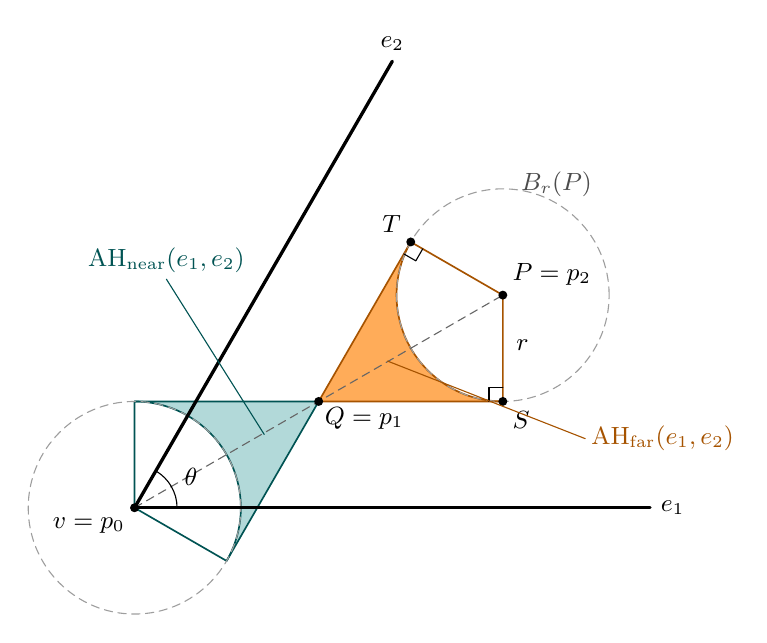
\begin{tikzpicture}[scale=1.35,line cap=round,line join=round,
  every node/.style={font=\small}]
  % r=1, theta=60 degrees; all coordinates follow Lemma 3.3.
  \pgfmathsetmacro{\cothalf}{sqrt(3)}
  \coordinate (V) at (0,0);
  \coordinate (Q) at (\cothalf,1);
  \coordinate (P) at ({2*\cothalf},2);
  \coordinate (S) at ({2*\cothalf},1);
  \coordinate (T) at ({1.5*\cothalf},2.5);
  \coordinate (U) at ({sqrt(3)/2},-0.5);
  \coordinate (W) at (0,1);
  \begin{scope}
    % The two exact congruent arrowheads, from their defining circular arcs.
    \fill[teal!30] (Q)--(U) arc[start angle=-30,end angle=90,radius=1]--cycle;
    \fill[orange!65] (Q)--(S) arc[start angle=-90,end angle=-210,radius=1]--cycle;
    \draw[teal!65!black,semithick] (V)--(U)--(Q)--(W)--cycle;
    \draw[teal!65!black,semithick] (U) arc[start angle=-30,end angle=90,radius=1];
    \draw[orange!65!black,semithick] (P)--(S)--(Q)--(T)--cycle;
    \draw[orange!65!black,semithick] (S) arc[start angle=-90,end angle=-210,radius=1];
    \draw[black!38,densely dashed,thin] (V) circle[radius=1];
    \draw[black!38,densely dashed,thin] (P) circle[radius=1];
    \draw[black!60,densely dashed,thin] (V)--(P);
    \draw[very thick] (V)--(4.85,0) node[right] {$e_1$};
    \draw[very thick] (V)--(60:4.85) node[above] {$e_2$};
    \draw[thin] (0.40,0) arc[start angle=0,end angle=60,radius=0.40];
    \node at (0.53,0.29) {$\theta$};
    % Right-angle markers in the far kite (S and T).
    \draw[thin] ($(S)+(-0.13,0)$)--($(S)+(-0.13,0.13)$)--($(S)+(0,0.13)$);
    \draw[thin] ($(T)+({-0.13*cos(60)},{-0.13*sin(60)})$)
      --($(T)+({0.13*cos(-30)-0.13*cos(60)},{0.13*sin(-30)-0.13*sin(60)})$)
      --($(T)+({0.13*cos(-30)},{0.13*sin(-30)})$);
    \foreach \pt in {V,Q,P,S,T} {\fill (\pt) circle[radius=1.2pt];}
    \node[below left] at (V) {$v=p_0$};
    \node[below right,inner sep=2pt] at (Q) {$Q=p_1$};
    \node[above right] at (P) {$P=p_2$};
    \node[below right] at (S) {$S$};
    \node[above left] at (T) {$T$};
    \node[right] at (3.50,1.53) {$r$};
    \node[above,black!70] at (3.97,2.83) {$B_r(P)$};
    \draw[teal!65!black,thin] (1.22,0.69)--(0.3,2.15)
      node[above,inner sep=2pt] {$\AHnear(e_1,e_2)$};
    \draw[orange!65!black,thin] (2.38,1.38)--(4.24,0.65)
      node[right,inner sep=2pt] {$\AHfar(e_1,e_2)$};
  \end{scope}
\end{tikzpicture}
\caption{The near (teal) and far (orange) arrowheads for an incident pair, drawn to scale for $\theta=\pi/3$. The far kite is $PSQT$, with $PS=PT=r$ and right angles at $S,T$; its arrowhead is the part of $K^\circ$ outside $B_r^\circ(P)$. The near kite has its distinguished disk centered at $v=p_0$. The two shaded regions are congruent.}
\label{fig:kite}
\end{figure}

\begin{lemma}[Arrowhead inclusion]\label{lem:arrowhead-inclusion}
Let $e_1,e_2$ be consecutive incident edges of a closed PL set $A$, with angle $\theta\in(0,\pi)$. Then
\[
\boxed{\AHfar(e_1,e_2)\subseteq E(A,r).}
\]
\end{lemma}

\begin{proof}
Put $P=p_2(e_1,e_2)$ and $Q=p_1(e_1,e_2)$. Suppose, toward a contradiction, that $x\in\AH(P,Q,r)$ but $x\notin E(A,r)$. Then some closed radius-$r$ ball $B_r(c)$ contains $x$ and is disjoint from $A_r$:
\begin{equation}\label{eq:AH-ball-disjoint}
B_r(c)\cap A_r=\varnothing.
\end{equation}
By \eqref{eq:ball-meets-offset-iff},
\begin{equation}\label{eq:c-distance-A}
d(c,A)>2r.
\end{equation}

Use the coordinates of \cref{lem:kite-coordinates}, and define
\[
n_1=(0,1),
\qquad
n_2=(\sin\theta,-\cos\theta).
\]
Since $x$ is in the open kite, \eqref{eq:kite1}--\eqref{eq:kite2} give
\begin{equation}\label{eq:nx-r}
\langle n_1,x\rangle>r,
\qquad
\langle n_2,x\rangle>r.
\end{equation}
Because $d(c,x)\le r$, both $\langle n_i,c\rangle$ are positive. Thus $c$ lies in the open wedge between the two rays. Write
\[
c=\rho(\cos\alpha,\sin\alpha),
\qquad 0<\alpha<\theta.
\]
We claim
\begin{equation}\label{eq:nc-2r}
\langle n_i,c\rangle>2r
\qquad(i=1,2).
\end{equation}
Indeed, by \eqref{eq:kite-norms}, $P$ is the kite vertex farthest from $v$, and hence
\[
d(v,c)\le d(v,x)+d(x,c)
\le2r\csc\frac\theta2+r<M.
\]
Whenever the orthogonal projection of $c$ onto an edge line points along the positive edge ray, that projection lies on the finite edge. If this happens for both edges, \eqref{eq:c-distance-A} immediately gives \eqref{eq:nc-2r}. If the projection onto $e_1$ is nonpositive, then $\alpha\ge\pi/2$, while the projection onto $e_2$ is positive. Hence
\[
\langle n_2,c\rangle=d(c,e_2)>2r.
\]
Moreover,
\[
\sin(\theta-\alpha)<\sin(\pi-\alpha)=\sin\alpha,
\]
so $\langle n_1,c\rangle>\langle n_2,c\rangle>2r$. The remaining case is symmetric.

By \cref{lem:kite-coordinates},
\[
\langle n_1,P\rangle=\langle n_2,P\rangle=2r.
\]
Thus
\[
\langle n_i,c-P\rangle>0
\qquad(i=1,2).
\]
Write
\[
c-P=\lambda_1\widehat e_1+\lambda_2\widehat e_2.
\]
Since
\[
\langle n_1,c-P\rangle=\lambda_2\sin\theta,
\qquad
\langle n_2,c-P\rangle=\lambda_1\sin\theta,
\]
we have $\lambda_1,\lambda_2>0$.

On the other hand, \eqref{eq:kite3}--\eqref{eq:kite4} imply
\[
\langle\widehat e_1,x-P\rangle<0,
\qquad
\langle\widehat e_2,x-P\rangle<0.
\]
Therefore
\[
\langle c-P,x-P\rangle<0.
\]
Consequently,
\[
\begin{aligned}
d(c,x)^2
&=\|(c-P)-(x-P)\|^2\\
&=\|c-P\|^2+\|x-P\|^2-2\langle c-P,x-P\rangle\\
&>\|x-P\|^2.
\end{aligned}
\]
Since $d(c,x)\le r$, it follows that $d(x,P)<r$, contradicting the defining condition $x\notin B_r^\circ(P)$ of the arrowhead.
\end{proof}

\begin{lemma}[Congruent arrowheads]\label{lem:congruent-arrowheads}
If $d(P,Q)=d(P',Q')$, then
\[
\AH(P,Q,r)\cong\AH(P',Q',r).
\]
In particular, for any distinct incident edges $e,f$,
\[
\boxed{\AHnear(e,f)\cong\AHfar(e,f).}
\]
\end{lemma}

\begin{proof}
The two right triangles forming the defining kite have one leg of length $r$ and common hypotenuse $PQ$. Hence equal values of $PQ$ give congruent kites, with the distinguished radius-$r$ disk carried to the corresponding disk. For the second assertion, $p_0,p_1,p_2$ are collinear and equally spaced, so
\[
d(p_0,p_1)=d(p_1,p_2).
\]
The straight-angle and disjoint cases are empty by convention.
\end{proof}
 \section{Characterization by consecutive arrowheads}\label{sec:characterization}

We now prove that, at the scale fixed in \cref{def:MR}, the only points added to $A_r$ are the far arrowheads associated to consecutive incident edges.

\subsection{Locating a point outside the ordinary offset}

\begin{lemma}[Nearest point at a vertex]\label{lem:nearest-vertex}
Let $A\subset\R^2$ be a closed PL set carried by $K$. Suppose
\[
x\in A_{2r}\setminus A_r
\]
and a nearest point of $A$ to $x$ is a vertex $v$. Then
\[
\boxed{d(x,\partial A_{2r})<r.}
\]
\end{lemma}

\begin{proof}
Put $\delta=d(x,A)=d(x,v)\in(r,2r]$, set
\[
u:=\frac{x-v}{\delta},
\qquad
z:=v+2ru.
\]
Then
\begin{equation}\label{eq:x-z-less-r}
d(x,z)=2r-\delta<r.
\end{equation}
We show $z\in\partial A_{2r}$.

If $\sigma$ is a simplex incident to $v$, then $v$ is a nearest point of the convex simplex $\sigma$ to $x$, so
\[
\langle u,a-v\rangle\le0
\qquad(a\in\sigma).
\]
Hence
\[
\|z-a\|^2
=4r^2+\|a-v\|^2-4r\langle u,a-v\rangle
\ge4r^2,
\]
and therefore $d(z,\sigma)\ge2r$. If $\sigma$ is not incident to $v$, then
\[
d(z,\sigma)\ge d(v,\sigma)-d(v,z)\ge M-2r>2r.
\]
Since $d(z,v)=2r$, we conclude
\[
d(z,A)=2r.
\]

For $t>0$, put $z_t=v+(2r+t)u$. The same normal-cone calculation gives $d(z_t,\sigma)>2r$ for every simplex incident to $v$. For a simplex not incident to $v$,
\[
d(z_t,\sigma)\ge M-(2r+t)>2r
\]
for all sufficiently small $t>0$. Thus $z_t\notin A_{2r}$ while $z\in A_{2r}$, proving $z\in\partial A_{2r}$. The result follows from \eqref{eq:x-z-less-r}.
\end{proof}

\begin{lemma}[Localization to an incident edge]\label{lem:localize-edge}
Let $A\subset\R^2$ be a closed PL set carried by $K$. Suppose
\[
x\in A_{2r}\setminus A_r,
\qquad
d(x,\partial A_{2r})\ge r,
\]
and let $p$ be a nearest point of $A$ to $x$. Assume $p\in\relint(e_1)$ for a boundary edge $e_1$ of $A$. Then there is a boundary edge $f\ne e_1$ sharing a vertex $v$ with $e_1$ and lying on the same side of the line through $e_1$ as $x$.

More precisely, coordinates may be chosen so that
\[
v=(0,0),
\qquad p=(a,0),
\qquad x=(a,\delta),
\]
with $e_1$ on the positive $X$-axis and $f$ making an angle $\phi\in(0,\pi)$ with $e_1$, such that
\begin{equation}\label{eq:a-phi-bound}
a\le2r\cot\frac\phi2,
\end{equation}
with strict inequality when $e_1$ and $f$ are consecutive.
\end{lemma}

\begin{proof}
Here $\delta=d(x,A)\in(r,2r]$. The hypothesis $d(x,\partial A_{2r})\ge r$ implies
\begin{equation}\label{eq:open-ball-inside-A2r}
B_r^\circ(x)\subseteq A_{2r};
\end{equation}
otherwise a segment from $x$ to a point outside $A_{2r}$ in $B_r^\circ(x)$ would meet $\partial A_{2r}$ at distance $<r$.

Because $p\in\relint(e_1)$ is the metric projection of $x$ onto the segment $e_1$, $x-p$ is perpendicular to $e_1$. Let
\[
n:=\frac{x-p}{\delta}.
\]
Choose $\eps_k\downarrow0$ with
\[
0<\eps_k<\min(\delta-r,R-r),
\]
and define
\[
y_k:=p+(2r+\eps_k)n.
\]
Then $d(x,y_k)<r$, so \eqref{eq:open-ball-inside-A2r} gives $y_k\in A_{2r}$.

Choose $q_k\in\partial A$ nearest to $y_k$. We claim
\begin{equation}\label{eq:yk-qk-2r}
d(y_k,q_k)\le2r.
\end{equation}
If $y_k\notin A$, a nearest point of $A$ lies on $\partial A$, and the claim follows from $y_k\in A_{2r}$. If $y_k\in A$, then the segment $[x,y_k]$ meets $\partial A$ because $x\notin A$; thus $d(y_k,\partial A)<r$.

It follows that
\[
d(p,q_k)\le d(p,y_k)+d(y_k,q_k)\le4r+\eps_k<4R.
\]
The point $q_k$ cannot be a vertex of $e_1$, because $p$ is the orthogonal projection of $y_k$ to $e_1$ and $d(y_k,p)=2r+\eps_k$. Nor can $q_k$ be any other vertex, since then $d(q_k,e_1)\ge M\ge8R$, contradicting $d(p,q_k)<4R$. Thus $q_k\in\relint(f_k)$ for a boundary edge $f_k\ne e_1$.

The edge $f_k$ must meet $e_1$: otherwise the disjoint-simplex separation gives $d(e_1,f_k)\ge M\ge8R$, whereas
\[
d(e_1,f_k)\le d(p,q_k)<4R.
\]
Passing to a subsequence, we may assume $f_k=f$ is fixed, meeting $e_1$ at a vertex $v$.

Choose coordinates with $v=(0,0)$, $e_1$ on the positive $X$-axis, and the positive $Y$-direction toward $x$. Then
\[
p=(a,0),
\qquad x=(a,\delta),
\qquad y_k=(a,2r+\eps_k).
\]
We first show that $f$ lies above the line of $e_1$. If instead it had direction $(\cos\beta,-\sin\beta)$ with $\beta\in(0,\pi]$, then $q_k$ being the interior orthogonal projection of $y_k$ onto $f$ would give
\[
a\cos\beta-(2r+\eps_k)\sin\beta>0.
\]
Hence $0<\beta<\pi/2$ and
\[
a>(2r+\eps_k)\tan\beta.
\]
The perpendicular distance from $y_k$ to $f$ would then satisfy
\[
\begin{aligned}
d(y_k,f)
&=a\sin\beta+(2r+\eps_k)\cos\beta\\
&>\frac{2r+\eps_k}{\cos\beta}>2r,
\end{aligned}
\]
contradicting \eqref{eq:yk-qk-2r}.

Let $\phi\in(0,\pi)$ be the angle from $e_1$ to $f$. Since $q_k$ is the orthogonal projection of $y_k$ onto $f$,
\[
\left|a\sin\phi-(2r+\eps_k)\cos\phi\right|\le2r.
\]
Letting $k\to\infty$ yields
\[
a\sin\phi\le2r(1+\cos\phi),
\]
which is \eqref{eq:a-phi-bound}.

Suppose now that $e_1,f$ are consecutive and equality holds in \eqref{eq:a-phi-bound}. Then
\[
p+2rn
=\left(2r\cot\frac\phi2,2r\right)
=p_2(e_1,f).
\]
Since $x=p+\delta n$ and $\delta>r$,
\[
d(x,p_2(e_1,f))=2r-\delta<r.
\]
By \cref{lem:palpha}, $p_2(e_1,f)\in A\cup\partial A_{2r}$. The first possibility contradicts $d(x,A)>r$, and the second contradicts $d(x,\partial A_{2r})\ge r$. Thus the inequality is strict for consecutive $e_1,f$.
\end{proof}

\begin{lemma}[Recognition of the arrowhead kite]\label{lem:recognize-kite}
Under the hypotheses and coordinates of \cref{lem:localize-edge}, let $e_2$ be the first incident edge encountered from $e_1$ toward $f$. Let $\theta\in(0,\pi)$ be the angle from $e_1$ to $e_2$. Then $e_1,e_2$ are consecutive. If $K$ is the right kite defining $\AHfar(e_1,e_2)$, then
\[
\boxed{x\in K^\circ.}
\]
\end{lemma}

\begin{proof}
Since $\theta\le\phi$ and $\cot(t/2)$ decreases on $(0,\pi)$, \cref{lem:localize-edge} gives
\begin{equation}\label{eq:a-theta-strict}
a<2r\cot\frac\theta2.
\end{equation}
Indeed, if $\theta<\phi$ the inequality is immediate; if $\theta=\phi$, then $f=e_2$ and the strict part of \cref{lem:localize-edge} applies.

Let
\[
\tau:=a\cos\theta+\delta\sin\theta
\]
be the signed coordinate of the orthogonal projection of $x$ onto the line of $e_2$. We claim $\tau>0$. If $\tau\le0$, then $\cos\theta<0$ and
\[
a\ge\frac{\delta\sin\theta}{-\cos\theta}
>\frac{r\sin\theta}{-\cos\theta}.
\]
For $\cos\theta<0$,
\[
\frac{\sin\theta}{-\cos\theta}
\ge2\frac{1+\cos\theta}{\sin\theta}
=2\cot\frac\theta2,
\]
so $a>2r\cot(\theta/2)$, contradicting \eqref{eq:a-theta-strict}. Thus $\tau>0$. Also
\[
0<\tau\le d(v,x)\le a+\delta<M\le\len(e_2),
\]
by \cref{lem:basic-separation}; hence the projection lies on the finite edge $e_2$.

Since $p=(a,0)$ is a nearest point of $A$ to $x=(a,\delta)$,
\[
d(x,e_2)\ge\delta.
\]
The perpendicular distance to $e_2$ is
\[
|a\sin\theta-\delta\cos\theta|.
\]
The expression inside the absolute value must be nonnegative: if
\[
\delta\cos\theta-a\sin\theta\ge\delta,
\]
then $\delta(\cos\theta-1)\ge a\sin\theta>0$, impossible. Therefore
\[
a\sin\theta-\delta\cos\theta=d(x,e_2)\ge\delta,
\]
which gives
\begin{equation}\label{eq:a-lower}
a\ge\delta\cot\frac\theta2.
\end{equation}
Combining \eqref{eq:a-theta-strict} and \eqref{eq:a-lower}, we obtain
\begin{equation}\label{eq:delta-less-2r}
\delta<2r.
\end{equation}

Put $h=\theta/2$. By \cref{lem:kite-coordinates}, membership of $x=(a,\delta)$ in $K^\circ$ is equivalent to
\begin{align*}
\delta&>r,\\
a\sin\theta-\delta\cos\theta&>r,\\
a&<2r\cot h,\\
a\cos\theta+\delta\sin\theta&<2r\cot h.
\end{align*}
The first three follow from $\delta>r$, the distance estimate above, and \eqref{eq:a-theta-strict}. For the fourth, use the identity
\begin{equation}\label{eq:cot-identity}
\cot h\cos\theta+\sin\theta=\cot h.
\end{equation}
If $\cos\theta\ge0$, then \eqref{eq:a-theta-strict} and \eqref{eq:delta-less-2r} give
\[
a\cos\theta+\delta\sin\theta
<2r(\cot h\cos\theta+\sin\theta)
=2r\cot h.
\]
If $\cos\theta<0$, \eqref{eq:a-lower} gives $a\cos\theta\le\delta\cot h\cos\theta$, and hence
\[
a\cos\theta+\delta\sin\theta
\le\delta(\cot h\cos\theta+\sin\theta)
=\delta\cot h<2r\cot h.
\]
Thus all four kite inequalities hold.
\end{proof}

\begin{figure}[!htbp]
\centering
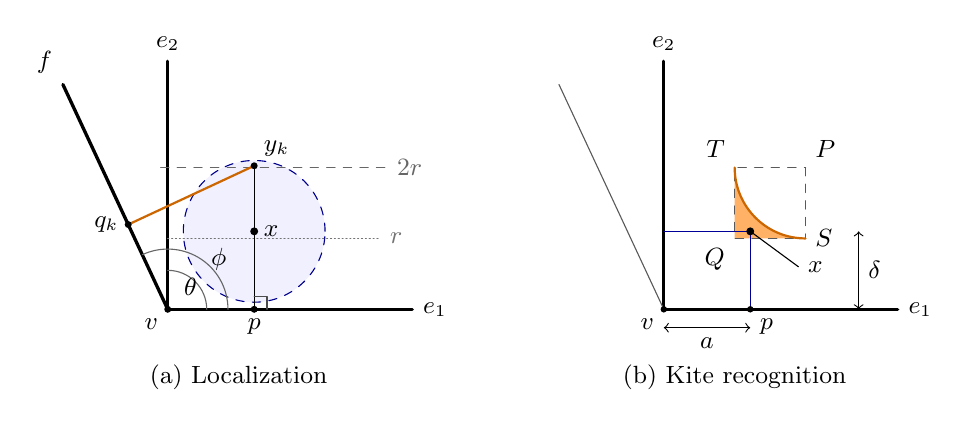
\begin{tikzpicture}[scale=0.9,line join=round,line cap=round,every node/.style={font=\small}]

  \begin{scope}
    \coordinate (v) at (0,0); \coordinate (p) at (1.22,0); \coordinate (x) at (1.22,1.10); \coordinate (y) at (1.22,2.025);
    \coordinate (q) at ({(1.22*cos(115)+2.025*sin(115))*cos(115)},{(1.22*cos(115)+2.025*sin(115))*sin(115)});
    \filldraw[fill=blue!6,draw=blue!55!black,dashed] (x) circle[radius=1];
    \draw[very thick] (v)--(3.45,0) node[right] {$e_1$};
    \draw[very thick] (v)--(0,3.5) node[above] {$e_2$};
    \draw[very thick] (v)--(115:3.5) node[above left] {$f$};
    \draw[black!60,dashed] (-.1,2)--(3.1,2) node[right] {$2r$};
    \draw[black!55,densely dotted] (0,1)--(3.0,1) node[right] {$r$};
    \draw[thin] (p)--(y); \draw[orange!80!black,thick] (y)--(q);
    \draw[black!70] (1.22,.18)--(1.40,.18)--(1.40,0);
    \draw[black!60] (.55,0) arc[start angle=0,end angle=90,radius=.55];
    \draw[black!60] (.85,0) arc[start angle=0,end angle=115,radius=.85];
    \node at (.32,.32) {$\theta$}; \node at (.72,.70) {$\phi$};
    \fill (p) circle[radius=1.4pt] node[below] {$p$}; \fill (v) circle[radius=1.4pt] node[below left] {$v$};
    \fill (x) circle[radius=1.6pt] node[right] {$x$}; \fill (y) circle[radius=1.4pt] node[above right] {$y_k$};
    \fill (q) circle[radius=1.4pt] node[left] {$q_k$};
    \node[anchor=north] at (1,-.65) {(a) Localization};
  \end{scope}
  \begin{scope}[xshift=7cm]
    \fill[orange!60] (1,1)--(2,1) arc[start angle=-90,end angle=-180,radius=1]--cycle;
    \draw[black!65,dashed] (2,2)--(2,1)--(1,1)--(1,2)--cycle;
    \draw[orange!80!black,thick] (2,1) arc[start angle=-90,end angle=-180,radius=1];
    \draw[very thick] (0,0)--(3.3,0) node[right] {$e_1$}; \draw[very thick] (0,0)--(0,3.5) node[above] {$e_2$};
    \draw[black!65,thin] (115:3.5)--(0,0);
    \draw[blue!60!black,thin] (1.22,0)--(1.22,1.10)--(0,1.10);
    \draw[<->,thin] (2.75,0)--(2.75,1.10) node[midway,right] {$\delta$};
    \draw[<->,thin] (0,-.26)--(1.22,-.26) node[midway,below] {$a$};
    \node[above right] at (2,2) {$P$}; \node[right] at (2,1) {$S$}; \node[below left] at (1,1) {$Q$}; \node[above left] at (1,2) {$T$};
    \fill (1.22,1.10) circle[radius=1.6pt]; \draw[thin] (1.22,1.10)--(1.9,.60) node[right] {$x$};
    \fill (1.22,0) circle[radius=1.3pt] node[below right] {$p$}; \fill (0,0) circle[radius=1.3pt] node[below left] {$v$};
    \node[anchor=north] at (1,-.65) {(b) Kite recognition};
  \end{scope}

\end{tikzpicture}
\caption{Local coordinates in Lemmas~\ref{lem:localize-edge} and~\ref{lem:recognize-kite}. In this example $r=1$, $a=1.22$, $\delta=1.10$, $\theta=90^\circ$, and $\phi=115^\circ$. Left: the test point $y_k$ lies on the perpendicular through $p$, inside $B_r(x)$ and within $2r$ of $f$; $q_k$ is its projection. Right: $e_2$ is the first intervening incident edge and the point $x$ lies strictly inside the far kite $PSQT$ and outside its radius-$r$ cutout. Only the local portions of the edges are drawn.}
\label{fig:localization-kite}
\end{figure}

\begin{lemma}[From the kite to the arrowhead]\label{lem:kite-to-arrowhead}
Let $x\in A_{2r}\setminus A_r$. Suppose $e_1,e_2$ are consecutive incident edges, $K$ is the defining kite of $\AHfar(e_1,e_2)$, and
\[
x\in K^\circ,
\qquad
d(x,\partial A_{2r})\ge r.
\]
Then
\[
\boxed{x\in\AHfar(e_1,e_2).}
\]
\end{lemma}

\begin{proof}
Put $P=p_2(e_1,e_2)$. By \cref{lem:palpha},
\[
P\in A\cup\partial A_{2r}.
\]
If $P\in A$, then $d(x,P)\ge d(x,A)>r$. If $P\in\partial A_{2r}$, then $d(x,P)\ge d(x,\partial A_{2r})\ge r$. Thus $x\notin B_r^\circ(P)$. Since $x\in K^\circ$, the definition of the arrowhead gives the conclusion.
\end{proof}

\subsection{Consecutive and exterior arrowheads}

\begin{definition}[Consecutive pair]\label{def:consecutive}
Two distinct incident edges $e_1,e_2$ are \emph{consecutive} if no third edge incident to their common vertex lies strictly inside their non-reflex angle.
\end{definition}

Define
\[
\AHcon(A)
:=
\bigcup_{\substack{e_1,e_2\in\Edges(A)\\
 e_1,e_2\text{ consecutive}}}
\AHfar(e_1,e_2).
\]

\begin{theorem}[Consecutive-arrowhead characterization]\label{thm:consecutive-characterization}
For every closed PL set $A\subset\R^2$ carried by $K$ and every $0<r<R$,
\[
\boxed{E(A,r)=A_r\cup\AHcon(A).}
\]
\end{theorem}

\begin{proof}
By \cref{lem:arrowhead-inclusion}, every consecutive far arrowhead is contained in $E(A,r)$, and $A_r\subseteq E(A,r)$. Thus the right-hand side is contained in the left-hand side.

Conversely, take $x\in E(A,r)\setminus A_r$. By \cref{thm:erosion-characterization}, $x\in A_{2r}\setminus A_r$. Choose a nearest boundary point $c\in\partial A_{2r}$ to $x$. Since \cref{lem:boundary-ball} excludes $E(A,r)$ from every $B_r^\circ(c)$,
\[
d(x,\partial A_{2r})\ge r.
\]
Let $p$ be a nearest point of $A$ to $x$. Such a point lies on $\partial A$. If $p$ is a vertex, \cref{lem:nearest-vertex} gives a contradiction. Hence $p\in\relint(e_1)$ for some boundary edge $e_1$.

Apply \cref{lem:localize-edge}, and let $e_2$ be the first incident edge toward the resulting edge $f$. Then $e_1,e_2$ are consecutive. By \cref{lem:recognize-kite}, $x$ lies in the open defining kite of $\AHfar(e_1,e_2)$, and \cref{lem:kite-to-arrowhead} yields
\[
x\in\AHfar(e_1,e_2)\subseteq\AHcon(A).
\]
\end{proof}

\begin{definition}[Exterior consecutive pair]\label{def:exterior}
A consecutive pair $e,g$ is \emph{exterior} if the two edges are not both boundary edges of a single two-simplex of $A$. Define
\[
\AHext(A)
:=
\bigcup_{\substack{e,g\text{ consecutive}\\e,g\text{ exterior}}}
\AHfar(e,g).
\]
\end{definition}

\begin{corollary}[Exterior consecutive refinement]\label{cor:exterior-characterization}
For every closed PL set $A$ carried by $K$,
\[
\boxed{E(A,r)=A_r\cup\AHext(A).}
\]
\end{corollary}

\begin{proof}
By \cref{thm:consecutive-characterization}, it suffices to show that if consecutive edges $e,g$ bound a two-simplex $\sigma$, then $\AHfar(e,g)\subseteq\sigma$. Let $z=e\cap g$ and let $h$ be the edge of $\sigma$ opposite $z$. Every point $x$ of the far arrowhead lies strictly inside the non-reflex sector between $e,g$ and satisfies
\[
d(x,z)<2r\csc\frac\theta2<M
\]
by \cref{lem:basic-separation}. Since $z\notin h$, $d(z,h)\ge M$. The ray from $z$ through $x$ meets $h$, but only at distance at least $M$ from $z$. Therefore $x$ occurs before that intersection and belongs to $\sigma$.
\end{proof}

\begin{lemma}[Exterior consecutive arrowheads avoid the offset]\label{lem:ext-avoid-offset}
If $e,g$ are an exterior consecutive pair of $A$, then
\[
\boxed{\AHfar(e,g)\cap A_r=\varnothing.}
\]
\end{lemma}

\begin{proof}
Let $z=e\cap g$ and let $\theta\in(0,\pi)$ be their angle. A point $x\in\AHfar(e,g)$ lies strictly inside the non-reflex sector and, by \eqref{eq:kite1}--\eqref{eq:kite2}, is at distance $>r$ from each boundary line of the sector. Moreover,
\[
d(x,z)<2r\csc\frac\theta2<\frac M2.
\]

If a simplex $\sigma$ of $A$ is not incident to $z$, then
\[
d(x,\sigma)\ge d(z,\sigma)-d(x,z)>\frac M2>r.
\]
If $\sigma$ is incident to $z$, consecutiveness implies that no other incident edge lies strictly inside the sector, and exteriority implies that $e,g$ do not bound a two-simplex there. The simplicial-complex intersection property therefore prevents any incident simplex from meeting the interior of that sector. Since $x$ lies more than $r$ from both boundary lines, $d(x,\sigma)>r$. Thus $d(x,A)>r$.
\end{proof}

\begin{lemma}[Disjoint consecutive arrowheads]\label{lem:disjoint-arrowheads}
Distinct far arrowheads arising from exterior consecutive pairs are pairwise disjoint. In addition, near arrowheads based at distinct vertices are disjoint.
\end{lemma}

\begin{proof}
Suppose first that two exterior consecutive far arrowheads are based at the same vertex. Each lies strictly inside the non-reflex sector determined by its defining pair, and the interiors of sectors belonging to distinct consecutive pairs are disjoint.

If the arrowheads are based at distinct vertices $z_1,z_2$, then for $x$ in the $i$th arrowhead,
\[
d(x,z_i)<2r\csc\frac{\theta_i}{2}<\frac M2.
\]
Thus a common point would imply
\[
M\le d(z_1,z_2)<\frac M2+\frac M2=M,
\]
a contradiction.

For a near arrowhead based at $z$, every vertex of its defining kite lies at distance at most
\[
d(z,p_1)=r\csc\frac\theta2<\frac M4
\]
from $z$, and hence so does the entire kite by convexity. Near arrowheads based at distinct vertices are therefore contained in disjoint $M/4$-balls.
\end{proof}

Combining the preceding two results gives the decomposition that drives the deletion argument.

\begin{corollary}[Disjoint exterior decomposition]\label{cor:disjoint-exterior}
For every closed PL set $A$ carried by $K$,
\[
\boxed{E(A,r)=A_r\sqcup\AHext(A).}
\]
Moreover, the arrowheads in the union defining $\AHext(A)$ are pairwise disjoint.
\end{corollary}
\begin{figure}[!htbp]
\centering
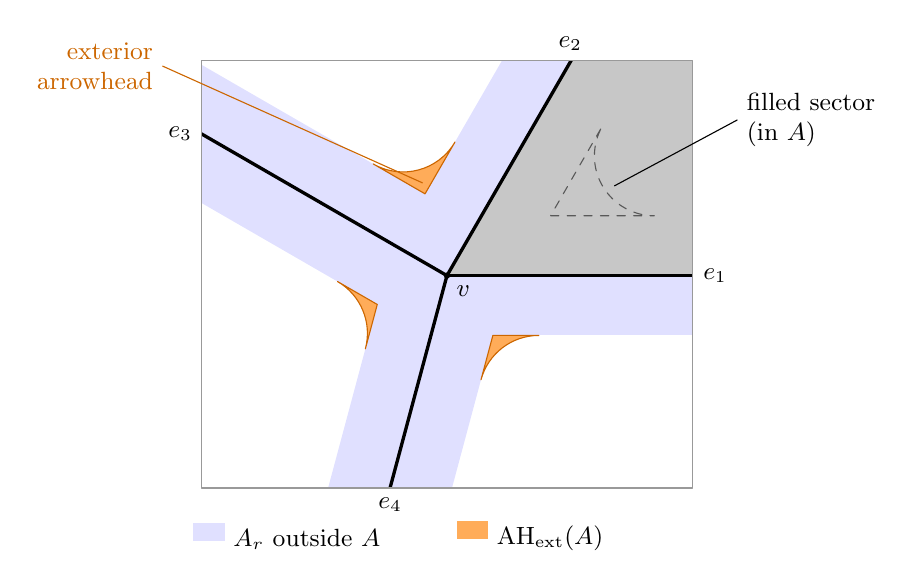
\begin{tikzpicture}[scale=0.76,line join=round,line cap=round,every node/.style={font=\small}]

  \begin{scope}
    \clip (-4.1,-3.55) rectangle (4.1,3.6);
    \fill[blue!12] (0,0) circle[radius=1];
    \foreach \a in {0,60,150,255}{\begin{scope}[rotate=\a]\fill[blue!12] (0,-1) rectangle (7,1);\end{scope}}
    \fill[black!22] (0,0)--(7,0)--(60:7)--cycle;
    
    \newcommand{\expatch}[3]{\begin{scope}[rotate=#1]\pgfmathsetmacro{\aa}{1/sin(#2)}\path[#3] (\aa,0)--({2*\aa+cos(270-#2)},{sin(270-#2)}) arc[start angle={270-#2},end angle={90+#2},radius=1]--cycle;\end{scope}}
    \expatch{30}{30}{draw=black!65,dashed,thin}
    \expatch{105}{45}{fill=orange!65,draw=orange!80!black,thin}
    \expatch{202.5}{52.5}{fill=orange!65,draw=orange!80!black,thin}
    \expatch{307.5}{52.5}{fill=orange!65,draw=orange!80!black,thin}
    \foreach \a in {0,60,150,255}{\draw[very thick] (0,0)--(\a:7);}
    \fill (0,0) circle[radius=1.5pt] node[below right] {$v$};
  \end{scope}
  \draw[black!40,thin] (-4.1,-3.55) rectangle (4.1,3.6);
  \node[anchor=west] at (4.12,0) {$e_1$}; \node[above] at (2.06,3.6) {$e_2$};
  \node[left] at (-4.1,2.37) {$e_3$}; \node[below] at (-.95,-3.55) {$e_4$};
  \draw[thin] (2.8,1.5)--(4.85,2.6) node[right,align=left] {filled sector\\(in $A$)};
  \draw[orange!80!black,thin] (-.41,1.55)--(-4.75,3.5) node[left,align=right] {exterior\\arrowhead};
  \node[anchor=west] at (-4.4,-4.35) {\tikz[baseline=-.5ex]\fill[blue!12] (0,0) rectangle (.4,.23); $A_r$ outside $A$};
  \node[anchor=west] at (0,-4.35) {\tikz[baseline=-.5ex]\fill[orange!65] (0,0) rectangle (.4,.23); $\AHext(A)$};

\end{tikzpicture}
\caption{Local example of Corollary~\ref{cor:disjoint-exterior} at a vertex with incident rays at $0^\circ,60^\circ,150^\circ,255^\circ$. The sector between $e_1$ and $e_2$ belongs to a two-simplex of $A$, so its far arrowhead (dashed outline) is already in $A$. The other three consecutive sectors have disjoint exterior far arrowheads (orange). The pair $e_1,e_3$ is not consecutive, since $e_2$ intervenes. The figure is a local view, with the incident edges continuing beyond the frame.}
\label{fig:exterior-decomposition}
\end{figure}

 \section{Deletion of an isolated open edge}\label{sec:edge-deletion}

Let $A\subset\R^2$ be a closed PL set carried by $K$, and let
\[
D=(v,w)
\]
be the relative interior of an edge of $K$ which is contained in $A$ but is not an edge of any two-simplex of $A$. Put
\[
B:=A\setminus D.
\]
Thus $D$ is an isolated one-dimensional stratum of $A$; simplices of $A$ may still meet $D$ at its endpoints.

The goal of this section is to prove
\begin{equation}\label{eq:segment-delta-target}
\boxed{
\Area\bigl(E(A,r)\setminus E(B,r)\bigr)
=2r\,\len(D)-\pi r^2.
}
\end{equation}

\subsection{Two edge offsets and an intervening edge}

\begin{lemma}[Intersection of two edge offsets]\label{lem:edge-offset-intersection}
Let $e,f$ be distinct finite edges meeting at a vertex $z$, with angle $\theta\in(0,\pi)$. Then, up to boundary,
\[
\boxed{
e_r\cap f_r
=
B_r(z)\cup\AHnear(e,f).
}
\]
Consequently,
\begin{equation}\label{eq:edge-offset-area}
\boxed{
\Area(e_r\cap f_r)
=
r^2\left(\cot\frac\theta2+\frac{\pi+\theta}{2}\right).
}
\end{equation}
\end{lemma}

\begin{proof}
Put $Q=p_1(e,f)$ and let $K_0$ be the closed right kite defining $\AH(z,Q,r)$. By \cref{lem:basic-separation},
\[
r\cot\frac\theta2<r\csc\frac\theta2<M,
\]
so the orthogonal projections of $Q$ onto the lines of $e$ and $f$ lie on the finite edges. Hence $d(Q,e)=d(Q,f)=r$, while the other three kite vertices lie in $B_r(z)$. Since $e_r\cap f_r$ is convex,
\[
K_0\subseteq e_r\cap f_r.
\]

Conversely, extend $e,f$ to rays $E,F$ from $z$. If
\[
y\in E_r\cap F_r\setminus B_r(z),
\]
then $z$ cannot be the nearest point of either ray to $y$, so the orthogonal projection of $y$ to each supporting line lies on the corresponding positive ray. The conditions $d(y,E),d(y,F)\le r$ are then exactly the four closed half-plane inequalities defining $K_0$. Therefore
\[
e_r\cap f_r=B_r(z)\cup K_0.
\]
Replacing $K_0\setminus B_r(z)$ by the open arrowhead changes only boundary sets.

The kite is the union of two congruent right triangles with legs $r$ and $r\cot(\theta/2)$, so
\[
\Area(K_0)=r^2\cot\frac\theta2.
\]
Its intersection with $B_r(z)$ is the radius-$r$ sector of angle $\pi-\theta$. Inclusion-exclusion yields \eqref{eq:edge-offset-area}.
\end{proof}

\begin{lemma}[Intervening edge]\label{lem:intervening-edge}
Let $D=(v,w)$ and $f=(v,u)$ be distinct incident edges making angle $\alpha\in(0,\pi)$. Let $\sigma$ be a simplex incident to $v$. Suppose $f$ lies angularly between $D$ and $\sigma$, and $\sigma$ lies in the same closed half-plane determined by the line of $D$ as $f$. Then
\[
\boxed{D_r\cap\sigma_r\subseteq D_r\cap f_r.}
\]
\end{lemma}

\begin{proof}
It suffices to show $D_r\cap\sigma_r\subseteq f_r$. Let $x\in D_r\cap\sigma_r$. If $d(x,v)\le r$, then $v\in f$ gives $x\in f_r$. Assume
\begin{equation}\label{eq:intervening-rho>r}
d(x,v)>r.
\end{equation}
Choose $y\in\sigma$ with $d(x,y)\le r$. Then $y\ne v$, and the polarization identity gives
\[
\langle x-v,y-v\rangle
=
\frac{d(x,v)^2+d(y,v)^2-d(x,y)^2}{2}>0.
\]
Thus the angle between $vx$ and $vy$ is less than $\pi/2$.

Choose coordinates with $v=0$, $D$ along angle $0$, and $f$ along angle $\alpha$. If $x$ lies on the $D$-side of the line containing $f$, the segment $[x,y]$ crosses the positive ray of $f$ at a point $z$, and $d(x,z)\le r$. If $x$ lies on the opposite side, choose $p\in\overline D$ with $d(x,p)\le r$; the positivity of $\langle x,y\rangle$ rules out the angular branch opposite $f$, so the segment $[p,x]$ crosses the positive ray of $f$ at a point $z$, again with $d(x,z)\le r$. Thus in either case
\begin{equation}\label{eq:intervening-z}
d(x,z)\le r
\end{equation}
for some $z$ on the positive ray through $f$.

Since $x$ lies within $r$ of the rays $D$ and $f$ and \eqref{eq:intervening-rho>r} excludes $v$ as the nearest point of either ray, both orthogonal projections are positive. Writing $\rho=d(x,v)$ and $\delta$ for the polar angle of $x-v$,
\[
\rho|\sin\delta|\le r,
\qquad
\rho|\sin(\delta-\alpha)|\le r.
\]
At least one of $|\delta|$ and $|\delta-\alpha|$ is at least $\alpha/2$, while both are $<\pi/2$. Hence
\begin{equation}\label{eq:intervening-rho-bound}
\rho\le r\csc\frac\alpha2.
\end{equation}
Combining \eqref{eq:intervening-z} and \eqref{eq:intervening-rho-bound},
\[
d(v,z)\le r\left(1+\csc\frac\alpha2\right)<M.
\]
Since every edge has length at least $M$, $z$ lies on the finite edge $f$. Therefore $d(x,f)\le r$.
\end{proof}

\begin{figure}[!htbp]
\centering
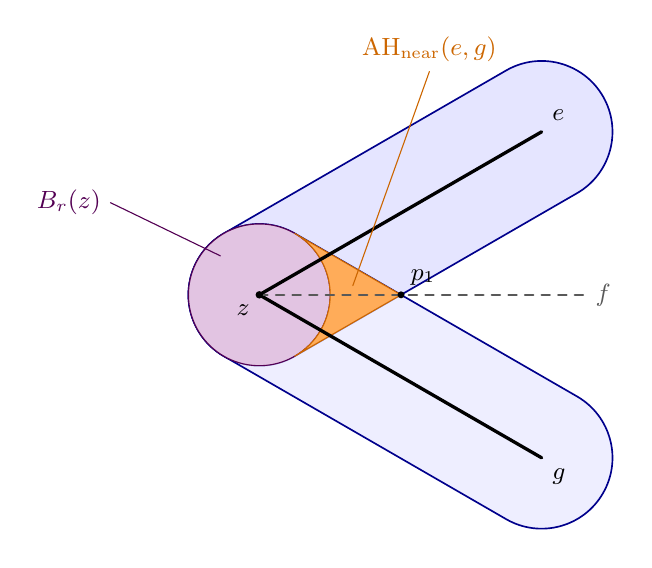
\begin{tikzpicture}[scale=0.9,line join=round,line cap=round,every node/.style={font=\small}]

  \newcommand{\capedge}[2]{\begin{scope}[rotate=#1]\path[#2] (0,-1)--(4.6,-1) arc[start angle=-90,end angle=90,radius=1]--(0,1) arc[start angle=90,end angle=270,radius=1]--cycle;\end{scope}}
  \capedge{30}{fill=blue!10,draw=blue!55!black,semithick}
  \capedge{-30}{fill=blue!10,draw=blue!55!black,semithick,fill opacity=.65}
  \filldraw[fill=violet!23,draw=violet!65!black] (0,0) circle[radius=1];
  \filldraw[fill=orange!65,draw=orange!80!black] (2,0)--(60:1) arc[start angle=60,end angle=-60,radius=1]--cycle;
  \draw[very thick] (0,0)--(30:4.6) node[above right] {$e$};
  \draw[very thick] (0,0)--(-30:4.6) node[below right] {$g$};
  \draw[black!65,dashed,thick] (0,0)--(4.6,0) node[right] {$f$};
  \fill (0,0) circle[radius=1.5pt] node[below left] {$z$};
  \fill (2,0) circle[radius=1.4pt] node[above right] {$p_1$};
  \draw[thin,violet!65!black] (-.55,.55)--(-2.1,1.3) node[left] {$B_r(z)$};
  \draw[thin,orange!80!black] (1.32,.13)--(2.4,3.15) node[above] {$\AHnear(e,g)$};

\end{tikzpicture}
\caption{Lemmas~\ref{lem:edge-offset-intersection} and~\ref{lem:intervening-edge} in a symmetric example: the two closed edge offsets at angle $60^\circ$ intersect in the disk $B_r(z)$ together with the near arrowhead (orange), up to boundary. The dashed ray is a possible intervening edge $f$; the intersection is also within its radius-$r$ offset. Here $r=1$; the finite edges are long enough that their other endpoints do not affect the depicted overlap.}
\label{fig:edge-offset-intersection}
\end{figure}

\subsection{Endpoint overlap geometry}

At an endpoint $z\in\{v,w\}$, let $e_z^+$ and $e_z^-$ be the first edges incident to $z$, other than $D$, encountered respectively counterclockwise and clockwise from the germ of $D$ at $z$, among edges making angle $<\pi$ with $D$ in the corresponding direction. Either may fail to exist. Define
\begin{align*}
\Lambda_z^\pm&:=\AHnear(D,e_z^\pm),
&\Lambda_z&:=\Lambda_z^+\cup\Lambda_z^-,\\
\Gamma_z^\pm&:=\AHfar(D,e_z^\pm),
&\Gamma_z&:=\Gamma_z^+\cup\Gamma_z^-.
\end{align*}
Nonexistent terms are omitted, and
\[
\Lambda:=\Lambda_v\cup\Lambda_w,
\qquad
\Gamma:=\Gamma_v\cup\Gamma_w.
\]

\begin{lemma}[Overlap with an isolated edge]\label{lem:isolated-edge-overlap}
Up to boundary,
\[
\boxed{
B_r\cap D_r
=
\{v,w\}_r\cup\Lambda,
}
\]
where $\{v,w\}_r=B_r(v)\cup B_r(w)$.
\end{lemma}

\begin{proof}
Because $2r<M$, the $r$-offset of a simplex disjoint from the closed edge $[v,w]$ is disjoint from $D_r$. Since no two-simplex of $A$ contains $D$ as an edge, the simplicial-complex intersection property excludes every simplex of $B$ from meeting the relative interior of $D$. Thus all contributions to $B_r\cap D_r$ come from the endpoints and simplices incident to them.

Fix $v$. If an incident simplex $\sigma$ lies entirely on one side of the line of $D$, the corresponding first edge $e_v^\pm$ lies angularly between $D$ and $\sigma$, so \cref{lem:intervening-edge} gives
\[
D_r\cap\sigma_r\subseteq D_r\cap(e_v^\pm)_r.
\]
If $\sigma$ crosses both sides of the line of $D$, split it along that line into two convex pieces and apply the same lemma on each side. If no qualifying edge exists on a side, the only contribution there is the endpoint disk; an edge exactly opposite $D$ likewise contributes only $B_r(v)$ to the overlap.

Thus the overlap is obtained from the endpoint disks and the intersections $D_r\cap(e_z^\pm)_r$. Applying \cref{lem:edge-offset-intersection} to each existing pair $(D,e_z^\pm)$ gives the stated formula up to boundary.
\end{proof}

\begin{corollary}[Overlap of near arrowheads]\label{cor:near-overlap}
Fix $z\in\{v,w\}$. Suppose both $e_z^+,e_z^-$ exist and $D$ lies strictly inside their non-reflex angle, which has size $<\pi$. Then, up to boundary,
\[
\boxed{
\Lambda_z^+\cap\Lambda_z^-
=
\AHnear(e_z^+,e_z^-).
}
\]
\end{corollary}

\begin{proof}
Since $D$ lies angularly between $e_z^+$ and $e_z^-$, \cref{lem:intervening-edge}, with $D$ as the intervening edge, gives
\[
(e_z^+)_r\cap(e_z^-)_r\subseteq D_r.
\]
Therefore
\[
D_r\cap(e_z^+)_r\cap(e_z^-)_r
=(e_z^+)_r\cap(e_z^-)_r.
\]
Apply \cref{lem:edge-offset-intersection} to the pairs $(D,e_z^+)$, $(D,e_z^-)$, and $(e_z^+,e_z^-)$, and remove the common endpoint disk; all changes occur only on boundaries.
\end{proof}

For later use define
\begin{equation}\label{eq:Xi-def}
\Xi_z:=\AHfar(e_z^+,e_z^-)
\end{equation}
when both edges exist and $D$ lies strictly inside their non-reflex angle. If that angle is $\pi$, the arrowhead is empty by convention. In every other configuration set $\Xi_z=\varnothing$, and put
\[
\Xi:=\Xi_v\cup\Xi_w.
\]

\begin{corollary}[Endpoint area cancellation in the non-reflex case]\label{cor:endpoint-cancellation}
If both $e_z^\pm$ exist and $D$ lies inside their non-reflex or straight angle, then
\[
\boxed{
\Area(\Gamma_z)
=
\Area(\Lambda_z)+\Area(\Xi_z).
}
\]
\end{corollary}

\begin{proof}
By \cref{lem:congruent-arrowheads}, each $\Gamma_z^\pm$ is congruent to $\Lambda_z^\pm$. The far arrowheads $\Gamma_z^+$ and $\Gamma_z^-$ lie on opposite sides of the line of $D$, hence are disjoint. If the angle between $e_z^+,e_z^-$ is $<\pi$, \cref{cor:near-overlap} and near--far congruence give
\[
\Area(\Lambda_z^+\cap\Lambda_z^-)=\Area(\Xi_z),
\]
and inclusion-exclusion yields the formula.

If the angle is $\pi$, then $\Xi_z=\varnothing$ and the offsets of the opposite edges intersect only in $B_r(z)$. The same edge-offset identities show that $\Lambda_z^+\cap\Lambda_z^-$ has area zero, so the two near-arrowhead areas add and again equal $\Area(\Gamma_z)$.
\end{proof}


\begin{figure}[htbp]
\centering
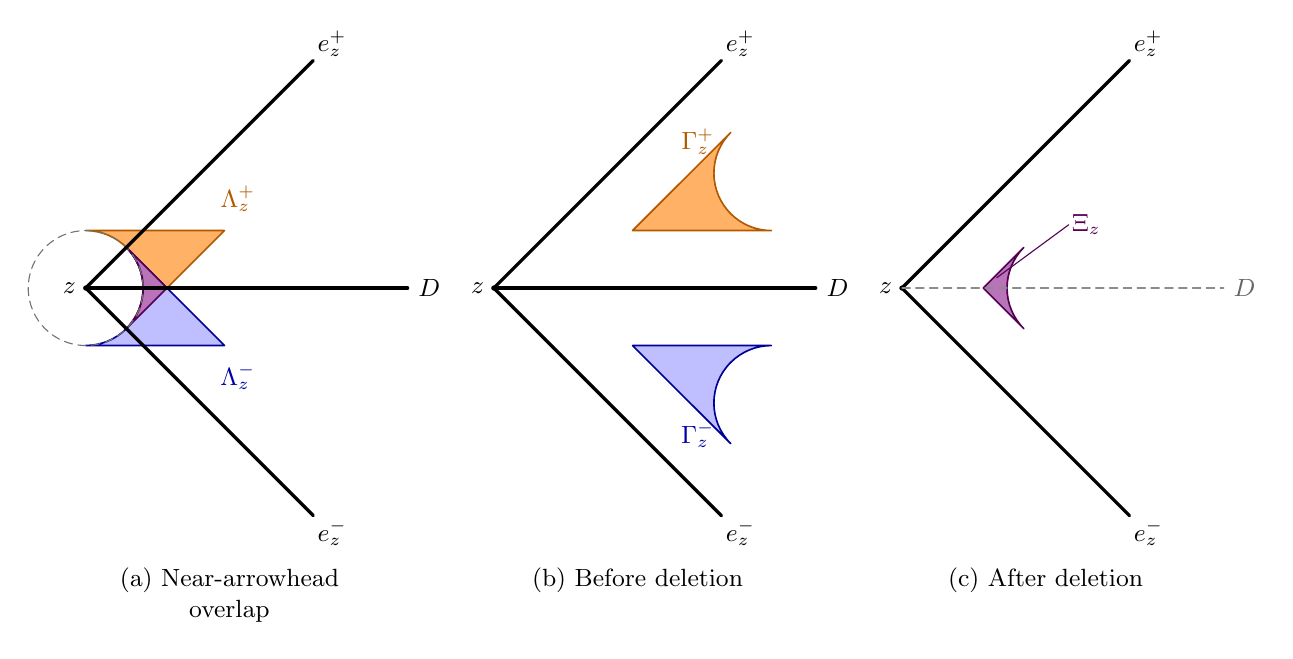
\begin{tikzpicture}[scale=0.73,line join=round,line cap=round,
  every node/.style={font=\small}]
  % A symmetric non-reflex example: incident rays at -45, 0, 45 degrees.
  % The unit radius is used in every panel. In local bisector coordinates,
  % the near tip is (csc h,0) and the far disk center is (2 csc h,0).
  \newcommand{\nearpatch}[2]{%
    \begin{scope}[rotate=#1]
      \path[#2] ({1/sin(22.5)},0)--(67.5:1)
        arc[start angle=67.5,end angle=-67.5,radius=1]--cycle;
    \end{scope}}
  \newcommand{\farpatch}[2]{%
    \begin{scope}[rotate=#1]
      \pgfmathsetmacro{\a}{1/sin(22.5)}
      \path[#2] (\a,0)--({2*\a+cos(247.5)},{sin(247.5)})
        arc[start angle=247.5,end angle=112.5,radius=1]--cycle;
    \end{scope}}
  \newcommand{\siderays}{%
    \draw[very thick] (0,0)--(45:5.6) node[above right,inner sep=1pt] {$e_z^+$};
    \draw[very thick] (0,0)--(-45:5.6) node[below right,inner sep=1pt] {$e_z^-$};
    \fill (0,0) circle[radius=1.3pt] node[left] {$z$};}
  \begin{scope}[xshift=0cm]
    \nearpatch{22.5}{fill=orange!60,draw=orange!70!black,semithick}
    \nearpatch{-22.5}{fill=blue!25,draw=blue!60!black,semithick}
    % Exact intersection: the near arrowhead for the outer pair (angle 90).
    \path[fill=violet!55,draw=violet!65!black,semithick]
      ({sqrt(2)},0)--(45:1) arc[start angle=45,end angle=-45,radius=1]--cycle;
    \draw[black!55,densely dashed] (0,0) circle[radius=1];
    \siderays
    \draw[very thick] (0,0)--(5.6,0) node[right] {$D$};
    \node[orange!70!black] at (2.65,1.55) {$\Lambda_z^+$};
    \node[blue!65!black] at (2.65,-1.55) {$\Lambda_z^-$};
    \node[anchor=north,align=center] at (2.5,-4.7) {(a) Near-arrowhead\\overlap};
  \end{scope}
  \begin{scope}[xshift=7.1cm]
    \farpatch{22.5}{fill=orange!60,draw=orange!70!black,semithick}
    \farpatch{-22.5}{fill=blue!25,draw=blue!60!black,semithick}
    \siderays
    \draw[very thick] (0,0)--(5.6,0) node[right] {$D$};
    \node[orange!70!black] at (3.55,2.55) {$\Gamma_z^+$};
    \node[blue!65!black] at (3.55,-2.55) {$\Gamma_z^-$};
    \node[anchor=north,align=center] at (2.5,-4.7) {(b) Before deletion};
  \end{scope}
  \begin{scope}[xshift=14.2cm]
    \path[fill=violet!55,draw=violet!65!black,semithick]
      ({sqrt(2)},0)--({2*sqrt(2)+cos(225)},{sin(225)})
      arc[start angle=225,end angle=135,radius=1]--cycle;
    \siderays
    \draw[black!45,densely dashed] (0,0)--(5.6,0) node[right,black!60] {$D$};
    \draw[violet!65!black,thin] (1.65,0.18)--(2.9,1.1)
      node[right,inner sep=1pt] {$\Xi_z$};
    \node[anchor=north,align=center] at (2.5,-4.7) {(c) After deletion};
  \end{scope}
\end{tikzpicture}
\caption{Endpoint cancellation in the non-reflex case, drawn to scale with $D$ bisecting the right angle between $e_z^+$ and $e_z^-$. (a) The violet region is the intersection $\Lambda_z^+\cap\Lambda_z^-$. (b) The two far arrowheads disappear when $D$ is deleted. (c) The newly consecutive pair has far arrowhead $\Xi_z$, congruent to the violet overlap in (a). Thus the total far-arrowhead area in (b), minus the new far-arrowhead area in (c), equals the area of the union of the two near arrowheads in (a). The dashed ray in (c) marks the deleted edge germ, not an edge of $B$.}
\label{fig:endpoint-cancellation}
\end{figure}

\begin{corollary}[Near arrowheads in the reflex case]\label{cor:reflex-near-disjoint}
Suppose both $e_z^\pm$ exist and $D$ lies strictly inside the reflex angle between them. Let $K_z^\pm$ be the defining kites of $\Lambda_z^\pm$. Then
\[
\boxed{K_z^+\cap K_z^-=\{z\}.}
\]
Consequently,
\[
\boxed{\Lambda_z^+\cap\Lambda_z^-=\varnothing}
\]
and
\[
\Area(\Lambda_z)=\Area(\Lambda_z^+)+\Area(\Lambda_z^-).
\]
\end{corollary}

\begin{proof}
Let
\[
\alpha=\angle(D,e_z^+),
\qquad
\beta=\angle(D,e_z^-)
\]
measured on their respective sides of $D$. The reflex hypothesis is
\[
\alpha+\beta>\pi.
\]
Suppose $x\ne z$ belongs to both kites, and let $\delta$ be the angle of $x-z$ measured from $D$, with $e_z^+$ at angle $\alpha$ and $e_z^-$ at angle $-\beta$. Every point of a near kite has nonnegative scalar projection onto both defining rays. Hence
\[
-\frac\pi2\le\delta\le\frac\pi2,
\]
\[
\alpha-\frac\pi2\le\delta\le\alpha+\frac\pi2,
\qquad
-\beta-\frac\pi2\le\delta\le-\beta+\frac\pi2.
\]
The last two intervals can intersect only if
\[
\alpha-\frac\pi2\le-\beta+\frac\pi2,
\]
i.e. $\alpha+\beta\le\pi$, a contradiction. Thus the two kites meet only at $z$. Each near arrowhead excludes $z$.
\end{proof}

\subsection{How exterior arrowheads change when \texorpdfstring{$D$}{D} is deleted}

\begin{lemma}[Consecutive-arrowhead change under deletion]\label{lem:arrowhead-change}
With the notation above,
\[
\boxed{
\AHext(B)
=
\bigl(\AHext(A)\setminus\Gamma\bigr)\sqcup\Xi.
}
\]
\end{lemma}

\begin{proof}
Fix an endpoint $z$. The only consecutive pairs of $A$ involving $D$ and having nonempty arrowheads are
\[
(D,e_z^+),
\qquad
(D,e_z^-),
\]
whenever the corresponding edges exist. Any farther edge has the appropriate first edge strictly between it and $D$, while an edge exactly opposite $D$ gives an empty arrowhead. Since $D$ is not an edge of any two-simplex, these pairs are exterior. Thus deleting $D$ removes precisely the terms comprising $\Gamma$.

Removing $D$ cannot destroy the consecutiveness of a pair not involving $D$. Conversely, a non-$D$ pair can become consecutive only if $D$ was the sole incident edge strictly inside its non-reflex angle. This happens exactly when the pair is $(e_z^+,e_z^-)$ and $D$ lies inside that non-reflex angle, which is precisely the case defining $\Xi_z$.

Any such newly consecutive pair is exterior in $B$. Indeed, if $e_z^+$ and $e_z^-$ were both sides of a two-simplex of $B$, the interior of that simplex near $z$ would intersect the germ of $D$, violating the simplicial-complex intersection property. Therefore the only new exterior consecutive arrowheads are the terms of $\Xi$.

Finally, the arrowheads appearing in $\AHext(B)$ are pairwise disjoint by \cref{lem:disjoint-arrowheads}, so the displayed union is disjoint.
\end{proof}

\subsection{Area of the deleted region}

\begin{theorem}[Area change for an isolated open edge]\label{thm:segment-delta}
Let
\[
\Delta:=E(A,r)\setminus E(B,r).
\]
Then
\[
\boxed{
\Area(\Delta)=2r\,\len(D)-\pi r^2.
}
\]
\end{theorem}

\begin{proof}
By \cref{cor:disjoint-exterior},
\[
E(A,r)=A_r\sqcup\AHext(A),
\qquad
E(B,r)=B_r\sqcup\AHext(B).
\]
Since $B\subseteq A$, \cref{lem:closure-monotone} gives $E(B,r)\subseteq E(A,r)$, so
\[
\Area(\Delta)=\Area(E(A,r))-\Area(E(B,r)).
\]
Using \cref{lem:arrowhead-change} and disjointness,
\begin{equation}\label{eq:Delta-area-decomp}
\Area(\Delta)
=
\Area(A_r)-\Area(B_r)
+
\Area(\Gamma)-\Area(\Xi).
\end{equation}

Now $A_r=B_r\cup D_r$. By \cref{lem:isolated-edge-overlap}, up to boundary,
\[
B_r\cap D_r=\{v,w\}_r\cup\Lambda.
\]
The endpoint disks are disjoint, and the separation estimates ensure that they meet the near-arrowhead pieces only on boundary. Hence
\[
\Area(B_r\cap D_r)=2\pi r^2+\Area(\Lambda).
\]
Since $D_r$ is the stadium around a segment of length $\len(D)$,
\[
\Area(D_r)=2r\,\len(D)+\pi r^2.
\]
Inclusion-exclusion therefore gives
\begin{equation}\label{eq:offset-area-change}
\Area(A_r)-\Area(B_r)
=
2r\,\len(D)-\pi r^2-\Area(\Lambda).
\end{equation}

It remains to compare arrowhead areas endpoint by endpoint. We claim that for each $z\in\{v,w\}$,
\begin{equation}\label{eq:endpoint-master}
\Area(\Gamma_z)-\Area(\Xi_z)=\Area(\Lambda_z).
\end{equation}
If both $e_z^\pm$ exist and $D$ lies inside their non-reflex or straight angle, this is \cref{cor:endpoint-cancellation}. If at most one of $e_z^\pm$ exists, then $\Xi_z=\varnothing$ and \eqref{eq:endpoint-master} follows directly from near--far congruence.

Finally suppose both $e_z^\pm$ exist and $D$ lies in their reflex angle. Then $\Xi_z=\varnothing$ by definition. By \cref{cor:reflex-near-disjoint},
\[
\Area(\Lambda_z)
=
\Area(\Lambda_z^+)+\Area(\Lambda_z^-).
\]
Near--far congruence gives the same sum for $\Gamma_z^\pm$, and these are distinct exterior consecutive far arrowheads, hence disjoint by \cref{lem:disjoint-arrowheads}. Thus $\Area(\Lambda_z)=\Area(\Gamma_z)$, proving \eqref{eq:endpoint-master} in the remaining case.

The far-arrowhead pieces based at $v$ and $w$ are disjoint, and \cref{lem:disjoint-arrowheads} also gives $\Lambda_v\cap\Lambda_w=\varnothing$. Summing \eqref{eq:endpoint-master} over the two endpoints yields
\begin{equation}\label{eq:arrowhead-area-cancel}
\Area(\Gamma)-\Area(\Xi)=\Area(\Lambda).
\end{equation}
Substitution of \eqref{eq:offset-area-change} and \eqref{eq:arrowhead-area-cancel} into \eqref{eq:Delta-area-decomp} proves the theorem.
\end{proof}
 \section{Proof of the planar PL extended Steiner formula}\label{sec:main-proof}

We now complete the proof of \cref{thm:main-intro}. The argument starts from a convex triangulation and removes the relatively open simplices which do not belong to $A$.

\subsection{Deleting an open triangle}

\begin{lemma}[Area change for an open triangle]\label{lem:triangle-deletion}
Let $A$ be a closed PL set carried by $K$, and let $D$ be the relative interior of a two-simplex $\overline D\subset A$. Put
\[
B:=A\setminus D.
\]
Then
\[
\boxed{
\Area\bigl(E(A,r)\setminus E(B,r)\bigr)
=
\Steiner(D,r).
}
\]
If $a=\Area(D)$ and $p$ is the perimeter of $\overline D$, this common value is
\[
a-pr+\pi r^2.
\]
\end{lemma}

\begin{proof}
Let
\[
T:=\{y\in\overline D:d(y,\partial D)\ge2r\}.
\]
For the present scale $T$ is a nonempty closed triangle parallel to $\overline D$. Indeed, every altitude of $\overline D$ is at least $M$. If $\rho_D$ is its inradius and $h_{\min}$ its least altitude, then
\[
\rho_D=\frac{2a}{p}\ge\frac{h_{\min}}3\ge\frac M3,
\]
while $2r<M/6$ by \cref{lem:basic-separation}.

We first identify the portion of the $2r$-parallel body which disappears when $D$ is removed. Since $B$ contains $\partial D$, for $y\in D$ one has
\[
d(y,B)=d(y,\partial D).
\]
For $y\notin D$, any segment from $y$ to a point of $D$ crosses $\partial D$ first, so if $y$ is within $2r$ of $D$, it is already within $2r$ of $B$. Hence
\begin{equation}\label{eq:A2r-minus-B2r-triangle}
A_{2r}\setminus B_{2r}=T^\circ,
\end{equation}
where $T^\circ$ denotes the interior of the inset triangle.

Let
\[
\Delta:=E(A,r)\setminus E(B,r).
\]
By \cref{thm:erosion-characterization}, a point $x\in E(A,r)$ lies outside $E(B,r)$ exactly when its closed radius-$r$ ball contains a point of $A_{2r}\setminus B_{2r}=T^\circ$. Thus
\begin{equation}\label{eq:triangle-delta-open-offset}
\Delta=\{x:d(x,T)<r\}=T_r^\circ.
\end{equation}
For the converse implicit in \eqref{eq:triangle-delta-open-offset}, if $d(x,T)<r$ then $x$ lies in $D$ because $T$ is at distance $2r$ from $\partial D$; hence $x\in A\subset E(A,r)$, while $B_r(x)$ meets $T^\circ\subset A_{2r}\setminus B_{2r}$, so $x\notin E(B,r)$. Therefore
\[
\Area(\Delta)=\Area(T_r).
\]

The inset triangle $T$ is homothetic to $\overline D$. Since its inradius is $\rho_D-2r$, its scale factor is
\[
\alpha
=\frac{\rho_D-2r}{\rho_D}
=1-\frac{pr}{a}.
\]
Consequently,
\[
\Area(T)=\alpha^2a
=a-2pr+\frac{p^2}{a}r^2,
\]
and
\[
\operatorname{Perimeter}(T)=\alpha p
=p-\frac{p^2}{a}r.
\]
By the classical Steiner formula for the convex triangle $T$,
\[
\begin{aligned}
\Area(T_r)
&=\Area(T)+\operatorname{Perimeter}(T)r+\pi r^2\\
&=a-pr+\pi r^2\\
&=\Steiner(D,r),
\end{aligned}
\]
where the last equality is \eqref{eq:S-open-triangle}.
\end{proof}

\begin{figure}[!htbp]
\centering
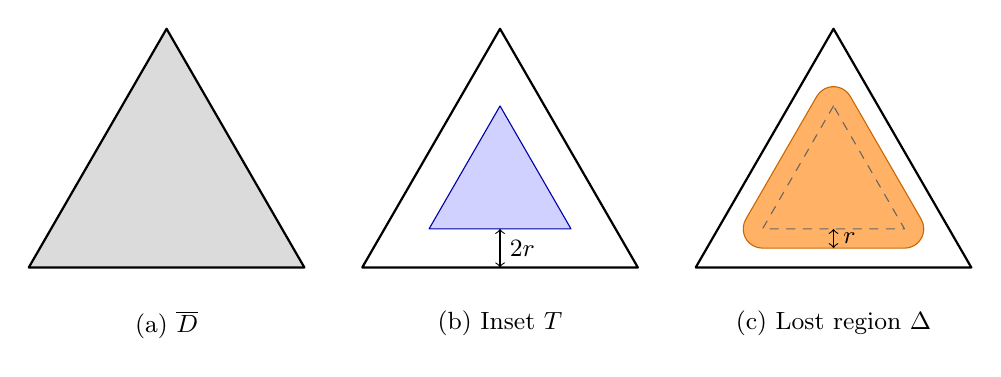
\begin{tikzpicture}[scale=0.7,line join=round,line cap=round,every node/.style={font=\small}]
  \begin{scope}[xshift=0.0cm]
    \fill[black!14] (0.000000,2.886751)--(-2.500000,-1.443376)--(2.500000,-1.443376)--cycle;
    \draw[thick] (0.000000,2.886751)--(-2.500000,-1.443376)--(2.500000,-1.443376)--cycle;
    \node[anchor=north] at (0,-2.05) {(a) $\overline D$};
  \end{scope}
  \begin{scope}[xshift=6.05cm]
    \filldraw[fill=blue!18,draw=blue!65!black] (0.000000,1.486751)--(-1.287564,-0.743376)--(1.287564,-0.743376)--cycle;
    \draw[thick] (0.000000,2.886751)--(-2.500000,-1.443376)--(2.500000,-1.443376)--cycle;
    \draw[<->,thin] (0,-1.4433756729740645)--(0,-0.7433756729740646) node[midway,right] {$2r$};
    \node[anchor=north] at (0,-2.05) {(b) Inset $T$};
  \end{scope}
  \begin{scope}[xshift=12.1cm]
    \filldraw[fill=orange!60,draw=orange!80!black] (0.303109,1.661751) arc[start angle=30,end angle=150,radius=0.35]--(-1.590673,-0.568376) arc[start angle=150,end angle=270,radius=0.35]--(1.287564,-1.093376) arc[start angle=270,end angle=390,radius=0.35]--cycle;
    \draw[black!60,dashed] (0.000000,1.486751)--(-1.287564,-0.743376)--(1.287564,-0.743376)--cycle;
    \draw[thick] (0.000000,2.886751)--(-2.500000,-1.443376)--(2.500000,-1.443376)--cycle;
    \draw[<->,thin] (0,-0.7433756729740646)--(0,-1.0933756729740645) node[midway,right] {$r$};
    \node[anchor=north] at (0,-2.05) {(c) Lost region $\Delta$};
  \end{scope}

\end{tikzpicture}
\caption{The construction in Lemma~\ref{lem:triangle-deletion}. From the closed triangle $\overline D$ (a), take the inset by $2r$ to obtain $T$ (b). The open radius-$r$ offset of $T$ is exactly the deleted extended-body region $\Delta=T_r^\circ$ (c), shown in orange; its boundary is drawn only to indicate the shape. All panels use the same scale.}
\label{fig:triangle-deletion}
\end{figure}

\subsection{Deleting an isolated vertex}

\begin{lemma}[Area change for an isolated vertex]\label{lem:vertex-deletion}
Let $A$ be a closed PL set carried by $K$, and suppose $z$ is an isolated vertex of $A$. Put $B=A\setminus\{z\}$. Then
\[
\boxed{
E(A,r)=E(B,r)\sqcup B_r(z)
}
\]
and hence
\[
\Area(E(A,r)\setminus E(B,r))=\pi r^2=\Steiner(\{z\},r).
\]
\end{lemma}

\begin{proof}
Because $z$ is isolated, no edge of $A$ is incident to it, so deleting $z$ changes none of the exterior consecutive arrowheads. Moreover, every simplex of $B$ is disjoint from $z$, and therefore
\[
d(z,B)\ge M>2r.
\]
Thus
\[
A_r=B_r\sqcup B_r(z).
\]
Using the disjoint exterior decomposition \cref{cor:disjoint-exterior} for $A$ and $B$ gives
\[
\begin{aligned}
E(A,r)
&=A_r\sqcup\AHext(A)\\
&=B_r(z)\sqcup B_r\sqcup\AHext(B)\\
&=B_r(z)\sqcup E(B,r).
\end{aligned}
\]
\end{proof}

\subsection{Deletion induction}

\begin{theorem}[Planar PL extended Steiner formula]\label{thm:main}
Let $A\subset\R^2$ be a nonempty closed PL set, let $K$ be a finite triangulation of $\conv(A)$ refining a simplicial representation of $A$, and let $R$ be defined by \cref{def:MR}. Then for every $0<r<R$,
\[
\boxed{
\Area(E(A,r))
=
\Area(A)+2\mu_1(A)r+\pi\chi(A)r^2
=
\Steiner(A,r).
}
\]
\end{theorem}

\begin{proof}
Let
\[
C:=\conv(A).
\]
By \cref{prop:convex-agreement},
\[
E(C,r)=C_r.
\]
The classical Steiner formula for compact convex sets therefore gives
\[
\Area(E(C,r))=\Steiner(C,r).
\]

Because $K$ refines a simplicial representation of $A$, the set $A$ is obtained from $C$ by deleting precisely those relatively open simplices of $K$ which do not belong to the subcomplex representing $A$. Perform these deletions in descending dimension:
\begin{enumerate}
\item first all missing open two-simplices;
\item then all missing open one-simplices;
\item finally all missing vertices.
\end{enumerate}
Write
\[
C=A_0\supset A_1\supset\cdots\supset A_N=A,
\qquad
A_{k+1}=A_k\setminus D_k,
\]
where each $D_k$ is the relatively open simplex removed at step $k$. With this order, every $A_k$ is closed. Moreover, when an open edge is removed, it is not an edge of any remaining two-simplex: if a two-simplex belonging to the target closed subcomplex remained, all of its faces would also belong to that subcomplex. Similarly, a vertex removed at the final stage is isolated.

Assume inductively that
\[
\Area(E(A_k,r))=\Steiner(A_k,r).
\]
Put
\[
\Delta_k:=E(A_k,r)\setminus E(A_{k+1},r).
\]
By monotonicity, $E(A_{k+1},r)\subseteq E(A_k,r)$, so
\begin{equation}\label{eq:induction-area-difference}
\Area(E(A_{k+1},r))
=
\Area(E(A_k,r))-\Area(\Delta_k).
\end{equation}
Since
\[
A_k=A_{k+1}\sqcup D_k,
\]
finite additivity of $\Steiner(\cdot,r)$ gives
\begin{equation}\label{eq:induction-S-difference}
\Steiner(A_{k+1},r)
=
\Steiner(A_k,r)-\Steiner(D_k,r).
\end{equation}
Thus it is enough to prove
\begin{equation}\label{eq:simplex-deletion-goal}
\Area(\Delta_k)=\Steiner(D_k,r).
\end{equation}

There are three cases. If $D_k$ is an open triangle, \eqref{eq:simplex-deletion-goal} is \cref{lem:triangle-deletion}. If $D_k$ is an open edge, the removal order makes it isolated from all two-simplices, and \cref{thm:segment-delta} gives
\[
\Area(\Delta_k)
=2r\,\len(D_k)-\pi r^2
=\Steiner(D_k,r)
\]
by \eqref{eq:S-open-edge}. If $D_k$ is a vertex, it is isolated at this stage and \cref{lem:vertex-deletion} gives \eqref{eq:simplex-deletion-goal}.

Therefore \eqref{eq:induction-area-difference} and \eqref{eq:induction-S-difference} propagate the desired identity from $A_k$ to $A_{k+1}$. Starting from the convex set $A_0=C$ and iterating finitely many times yields the result for $A_N=A$.
\end{proof}

\begin{figure}[!htbp]
\centering
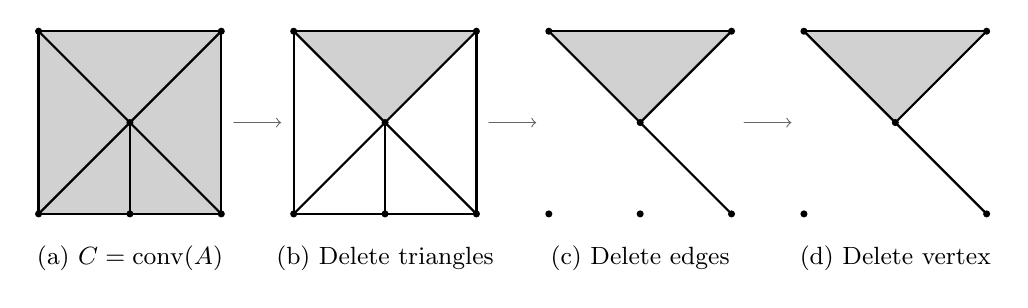
\begin{tikzpicture}[scale=0.8,line join=round,line cap=round,every node/.style={font=\small}]
  \begin{scope}[xshift=0.0cm]
    \coordinate (a) at (-1.45,-1.45);
    \coordinate (b) at (1.45,-1.45);
    \coordinate (c) at (1.45,1.45);
    \coordinate (d) at (-1.45,1.45);
    \coordinate (o) at (0,0);
    \coordinate (m) at (0,-1.45);
    \fill[black!18] (o)--(a)--(m)--cycle;
    \fill[black!18] (o)--(m)--(b)--cycle;
    \fill[black!18] (o)--(b)--(c)--cycle;
    \fill[black!18] (o)--(c)--(d)--cycle;
    \fill[black!18] (o)--(d)--(a)--cycle;
    \draw[thick] (a)--(m);
    \draw[thick] (m)--(b);
    \draw[thick] (b)--(c);
    \draw[thick] (c)--(d);
    \draw[thick] (d)--(a);
    \draw[thick] (a)--(o);
    \draw[thick] (b)--(o);
    \draw[thick] (c)--(o);
    \draw[thick] (d)--(o);
    \draw[thick] (m)--(o);
    \fill (a) circle[radius=1.6pt];
    \fill (b) circle[radius=1.6pt];
    \fill (c) circle[radius=1.6pt];
    \fill (d) circle[radius=1.6pt];
    \fill (o) circle[radius=1.6pt];
    \fill (m) circle[radius=1.6pt];
    \node[anchor=north] at (0,-1.8) {(a) $C=\conv(A)$};
  \end{scope}
  \begin{scope}[xshift=4.05cm]
    \coordinate (a) at (-1.45,-1.45);
    \coordinate (b) at (1.45,-1.45);
    \coordinate (c) at (1.45,1.45);
    \coordinate (d) at (-1.45,1.45);
    \coordinate (o) at (0,0);
    \coordinate (m) at (0,-1.45);
    \fill[black!18] (o)--(c)--(d)--cycle;
    \draw[thick] (a)--(m);
    \draw[thick] (m)--(b);
    \draw[thick] (b)--(c);
    \draw[thick] (c)--(d);
    \draw[thick] (d)--(a);
    \draw[thick] (a)--(o);
    \draw[thick] (b)--(o);
    \draw[thick] (c)--(o);
    \draw[thick] (d)--(o);
    \draw[thick] (m)--(o);
    \fill (a) circle[radius=1.6pt];
    \fill (b) circle[radius=1.6pt];
    \fill (c) circle[radius=1.6pt];
    \fill (d) circle[radius=1.6pt];
    \fill (o) circle[radius=1.6pt];
    \fill (m) circle[radius=1.6pt];
    \node[anchor=north] at (0,-1.8) {(b) Delete triangles};
  \end{scope}
  \begin{scope}[xshift=8.1cm]
    \coordinate (a) at (-1.45,-1.45);
    \coordinate (b) at (1.45,-1.45);
    \coordinate (c) at (1.45,1.45);
    \coordinate (d) at (-1.45,1.45);
    \coordinate (o) at (0,0);
    \coordinate (m) at (0,-1.45);
    \fill[black!18] (o)--(c)--(d)--cycle;
    \draw[thick] (c)--(d);
    \draw[thick] (c)--(o);
    \draw[thick] (d)--(o);
    \draw[thick] (b)--(o);
    \fill (a) circle[radius=1.6pt];
    \fill (b) circle[radius=1.6pt];
    \fill (c) circle[radius=1.6pt];
    \fill (d) circle[radius=1.6pt];
    \fill (o) circle[radius=1.6pt];
    \fill (m) circle[radius=1.6pt];
    \node[anchor=north] at (0,-1.8) {(c) Delete edges};
  \end{scope}
  \begin{scope}[xshift=12.149999999999999cm]
    \coordinate (a) at (-1.45,-1.45);
    \coordinate (b) at (1.45,-1.45);
    \coordinate (c) at (1.45,1.45);
    \coordinate (d) at (-1.45,1.45);
    \coordinate (o) at (0,0);
    \coordinate (m) at (0,-1.45);
    \fill[black!18] (o)--(c)--(d)--cycle;
    \draw[thick] (c)--(d);
    \draw[thick] (c)--(o);
    \draw[thick] (d)--(o);
    \draw[thick] (b)--(o);
    \fill (a) circle[radius=1.6pt];
    \fill (b) circle[radius=1.6pt];
    \fill (c) circle[radius=1.6pt];
    \fill (d) circle[radius=1.6pt];
    \fill (o) circle[radius=1.6pt];
    \node[anchor=north] at (0,-1.8) {(d) Delete vertex};
  \end{scope}
  \draw[->,black!60] (1.65,0)--(2.4,0);
  \draw[->,black!60] (5.699999999999999,0)--(6.449999999999999,0);
  \draw[->,black!60] (9.75,0)--(10.5,0);

\end{tikzpicture}
\caption{Example of the deletion order in the proof of Theorem~\ref{thm:main}. The target $A$ (d) consists of a closed triangle, an attached edge and an isolated corner vertex; its convex hull is the square $C$ (a). Remove the four unwanted relatively open triangles (b), then the six unwanted relatively open edges (c), and finally the unwanted isolated bottom-edge midpoint (d). Every intermediate set is closed.}
\label{fig:deletion-induction}
\end{figure}

\begin{remark}[Role of the radius]\label{rem:radius}
The explicit $R$ above is chosen for uniformity across all intermediate subcomplexes of $K$. It is not asserted to be optimal. Its purpose is to guarantee that all local arrowhead and separation arguments remain confined to the incident simplices which generate them.
\end{remark}
 \section{Frontier extension to nonclosed sets}\label{sec:frontier}

The preceding theorem is a closed-set result. The passage from closed to nonclosed sets is formal and does not depend on PL geometry beyond the finite termination of an appropriate frontier filtration.

For a set $A$ define its \emph{missing frontier}
\[
F(A):=\overline A\setminus A,
\]
and recursively
\[
F^0(A):=A,
\qquad
F^{k+1}(A):=F(F^k(A)).
\]
Also write
\[
A^r:=E(A,r).
\]

\begin{theorem}[Frontier extension principle]\label{thm:frontier-extension}
Fix $r\ge0$. Let $\mathcal C$ be a class of subsets of $\R^n$ such that for every $A\in\mathcal C$:
\begin{enumerate}
\item $\overline A\in\mathcal C$;
\item $F(A)=\overline A\setminus A\in\mathcal C$;
\item the frontier iteration terminates: $F^N(A)=\varnothing$ for some finite $N$.
\end{enumerate}
Let $\Steiner(\cdot,r)$ be a finitely additive valuation on $\mathcal C$. Assume that for every closed $C\in\mathcal C$ the closed-set volume identity
\begin{equation}\label{eq:abstract-closed-identity}
\boxed{
\Vol_n(E(C,r))=\Steiner(C,r)
}
\end{equation}
holds. Then for every $A\in\mathcal C$,
\begin{equation}\label{eq:frontier-alternating-sum}
\boxed{
\Steiner(A,r)
=
\sum_{k=0}^{N-1}(-1)^k
\Vol_n\bigl(F^k(A)^r\bigr).
}
\end{equation}

Moreover, the extended bodies form a nested chain
\[
F^0(A)^r\supseteq F^1(A)^r\supseteq\cdots\supseteq F^N(A)^r=\varnothing.
\]
Hence the alternating sum is the ordinary volume of the physical region
\begin{equation}\label{eq:physical-frontier-region}
\boxed{
\calE(A,r)
:=
\bigsqcup_{j\ge0}
\left(
F^{2j}(A)^r\setminus F^{2j+1}(A)^r
\right),
}
\end{equation}
where the union is finite. In particular,
\begin{equation}\label{eq:physical-frontier-volume}
\boxed{
\Vol_n(\calE(A,r))=\Steiner(A,r).
}
\end{equation}
\end{theorem}

\begin{proof}
For any $C\in\mathcal C$,
\[
\overline C=C\sqcup F(C).
\]
Finite additivity therefore gives
\begin{equation}\label{eq:S-frontier-one-step}
\Steiner(C,r)
=
\Steiner(\overline C,r)-\Steiner(F(C),r).
\end{equation}
By \cref{lem:closure-monotone}, $E(C,r)=E(\overline C,r)$. Since $\overline C$ is closed, \eqref{eq:abstract-closed-identity} turns \eqref{eq:S-frontier-one-step} into
\begin{equation}\label{eq:frontier-recursion}
\Steiner(C,r)
=
\Vol_n(C^r)-\Steiner(F(C),r).
\end{equation}
Apply \eqref{eq:frontier-recursion} successively to
\[
A,F(A),F^2(A),\ldots,F^{N-1}(A).
\]
Because $F^N(A)=\varnothing$, the recursion terminates and yields \eqref{eq:frontier-alternating-sum}.

For the physical form, observe that
\[
F^{k+1}(A)\subseteq\overline{F^k(A)}.
\]
Monotonicity and closure invariance of $E$ imply
\[
F^{k+1}(A)^r
\subseteq
E(\overline{F^k(A)},r)
=F^k(A)^r.
\]
Thus the sets in the filtration are nested. The differences in \eqref{eq:physical-frontier-region} are consequently pairwise disjoint, and
\[
\begin{aligned}
\Vol_n(\calE(A,r))
&=\sum_{j\ge0}
\left[
\Vol_n(F^{2j}(A)^r)
-
\Vol_n(F^{2j+1}(A)^r)
\right]\\
&=\sum_{k=0}^{N-1}(-1)^k\Vol_n(F^k(A)^r)\\
&=\Steiner(A,r).
\end{aligned}
\]
\end{proof}

\begin{figure}[!htbp]
\centering
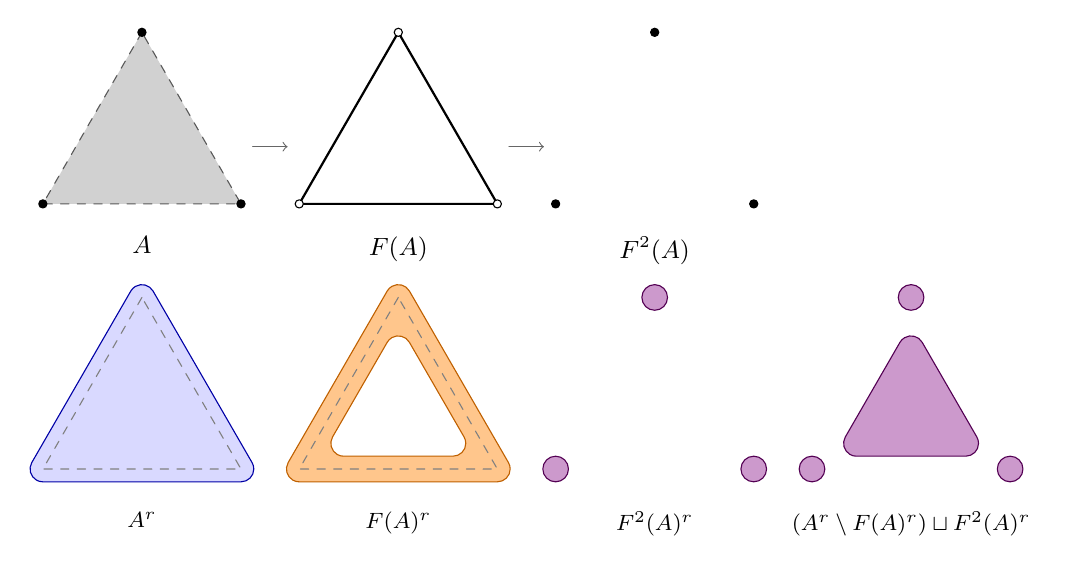
\begin{tikzpicture}[scale=0.74,line join=round,line cap=round,every node/.style={font=\small}]
  \begin{scope}[xshift=0.0cm,yshift=4.55cm]
    \fill[black!18] (0.000000,1.962991)--(-1.700000,-0.981495)--(1.700000,-0.981495)--cycle;\draw[black!65,dashed] (0.000000,1.962991)--(-1.700000,-0.981495)--(1.700000,-0.981495)--cycle;
    \filldraw[fill=black,draw=black] (0.000000,1.962991) circle[radius=2pt];
    \filldraw[fill=black,draw=black] (-1.700000,-0.981495) circle[radius=2pt];
    \filldraw[fill=black,draw=black] (1.700000,-0.981495) circle[radius=2pt];
    \node[anchor=north] at (0,-1.38) {$A$};
  \end{scope}
  \begin{scope}[xshift=4.4cm,yshift=4.55cm]
    \draw[thick] (0.000000,1.962991)--(-1.700000,-0.981495)--(1.700000,-0.981495)--cycle;
    \filldraw[fill=white,draw=black] (0.000000,1.962991) circle[radius=2pt];
    \filldraw[fill=white,draw=black] (-1.700000,-0.981495) circle[radius=2pt];
    \filldraw[fill=white,draw=black] (1.700000,-0.981495) circle[radius=2pt];
    \node[anchor=north] at (0,-1.38) {$F(A)$};
  \end{scope}
  \begin{scope}[xshift=8.8cm,yshift=4.55cm]
    \filldraw[fill=black,draw=black] (0.000000,1.962991) circle[radius=2pt];
    \filldraw[fill=black,draw=black] (-1.700000,-0.981495) circle[radius=2pt];
    \filldraw[fill=black,draw=black] (1.700000,-0.981495) circle[radius=2pt];
    \node[anchor=north] at (0,-1.38) {$F^2(A)$};
  \end{scope}
  \begin{scope}[xshift=0.0cm]
    \filldraw[fill=blue!15,draw=blue!65!black] (0.190526,2.072991) arc[start angle=30,end angle=150,radius=0.22]--(-1.890526,-0.871495) arc[start angle=150,end angle=270,radius=0.22]--(1.700000,-1.201495) arc[start angle=270,end angle=390,radius=0.22]--cycle;
    \draw[black!50,dashed,thin] (0.000000,1.962991)--(-1.700000,-0.981495)--(1.700000,-0.981495)--cycle;
    \node[anchor=north,font=\footnotesize] at (0,-1.55) {$A^r$};
  \end{scope}
  \begin{scope}[xshift=4.4cm]
    \filldraw[fill=orange!45,draw=orange!75!black,even odd rule] (0.190526,2.072991) arc[start angle=30,end angle=150,radius=0.22]--(-1.890526,-0.871495) arc[start angle=150,end angle=270,radius=0.22]--(1.700000,-1.201495) arc[start angle=270,end angle=390,radius=0.22]--cycle (0.190526,1.192991) arc[start angle=30,end angle=150,radius=0.22]--(-1.128423,-0.431495) arc[start angle=150,end angle=270,radius=0.22]--(0.937898,-0.761495) arc[start angle=270,end angle=390,radius=0.22]--cycle;
    \draw[black!50,dashed,thin] (0.000000,1.962991)--(-1.700000,-0.981495)--(1.700000,-0.981495)--cycle;
    \node[anchor=north,font=\footnotesize] at (0,-1.55) {$F(A)^r$};
  \end{scope}
  \begin{scope}[xshift=8.8cm]
    \filldraw[fill=violet!40,draw=violet!65!black] (0.000000,1.962991) circle[radius=0.22];
    \filldraw[fill=violet!40,draw=violet!65!black] (-1.700000,-0.981495) circle[radius=0.22];
    \filldraw[fill=violet!40,draw=violet!65!black] (1.700000,-0.981495) circle[radius=0.22];
    \node[anchor=north,font=\footnotesize] at (0,-1.55) {$F^2(A)^r$};
  \end{scope}
  \begin{scope}[xshift=13.200000000000001cm]
    \filldraw[fill=violet!40,draw=violet!65!black] (0.190526,1.192991) arc[start angle=30,end angle=150,radius=0.22]--(-1.128423,-0.431495) arc[start angle=150,end angle=270,radius=0.22]--(0.937898,-0.761495) arc[start angle=270,end angle=390,radius=0.22]--cycle;
    \filldraw[fill=violet!40,draw=violet!65!black] (0.000000,1.962991) circle[radius=0.22];
    \filldraw[fill=violet!40,draw=violet!65!black] (-1.700000,-0.981495) circle[radius=0.22];
    \filldraw[fill=violet!40,draw=violet!65!black] (1.700000,-0.981495) circle[radius=0.22];
    \node[anchor=north,font=\footnotesize] at (0,-1.55) {$(A^r\setminus F(A)^r)\sqcup F^2(A)^r$};
  \end{scope}
  \draw[->,black!60] (1.9,4.55)--(2.5,4.55);
  \draw[->,black!60] (6.300000000000001,4.55)--(6.9,4.55);

\end{tikzpicture}
\caption{Example of Corollary~\ref{cor:nonclosed-planar}: $A$ is an open equilateral triangle together with its three vertices. Its missing frontier consists of the three open edges; the next missing frontier is the three vertices. The lower row shows the corresponding extended bodies and the final physical region (violet), namely the rounded inset triangle together with three vertex disks. Dashed edges in the first panel are excluded from $A$; open circles denote excluded endpoints. Boundaries of the shaded regions are indicated for visibility.}
\label{fig:frontier-filtration}
\end{figure}

\begin{corollary}[Arbitrary planar PL sets]\label{cor:nonclosed-planar}
Let $A\subset\R^2$ be an arbitrary PL set, and choose a finite complex carrying $\overline A$. Suppose $0<r<R$ is small enough that \cref{thm:main} applies to every closed PL set occurring in the frontier filtration. Then
\[
F^3(A)=\varnothing
\]
and
\begin{equation}\label{eq:planar-frontier-sum}
\boxed{
\Steiner(A,r)
=
\Area(A^r)
-
\Area(F(A)^r)
+
\Area(F^2(A)^r).
}
\end{equation}
Moreover,
\[
F^2(A)^r\subseteq F(A)^r\subseteq A^r,
\]
so the same number is realized as the area of a single region:
\begin{equation}\label{eq:planar-physical-form}
\boxed{
\Area\left(
[A^r\setminus F(A)^r]\sqcup F^2(A)^r
\right)
=
\Steiner(A,r).
}
\end{equation}
Equivalently,
\begin{equation}\label{eq:planar-physical-form2}
\boxed{
\Area\left(
A^r\setminus\bigl(F(A)^r\setminus F^2(A)^r\bigr)
\right)
=
\Steiner(A,r).
}
\end{equation}
\end{corollary}

\begin{proof}
For a finite planar PL set, every nonempty application of $F$ removes present strata and leaves only missing faces of strictly smaller dimension. Thus
\[
\dim F(A)\le1,
\qquad
\dim F^2(A)\le0.
\]
A zero-dimensional finite PL set is closed, so $F^3(A)=\varnothing$. The closed members of this finite filtration are carried by the same ambient complex, so the global radius of \cref{def:MR} may be chosen uniformly. Apply \cref{thm:frontier-extension} and then use the nesting to obtain the physical forms.
\end{proof}
 \section{Remarks and further directions}\label{sec:outlook}

The definition of $E(A,r)$ is not PL-specific and makes sense in every Euclidean dimension. The planar PL proof above uses the finite local angular geometry of a simplicial complex in an essential way, but the identity
\[
E(A,r)=A_{2r}\ominus B_r
\]
suggests several directions in which the construction can be studied independently of that proof.

First, on classes for which curvature or intrinsic-volume valuations admit stable approximation, it is natural to ask whether the closed-set identity persists beyond PL sets, either exactly for sufficiently small $r$ or asymptotically as $r\downarrow0$. Second, in higher dimensions one may ask whether the corresponding volume is governed by the full intrinsic-volume polynomial
\[
\Vol_n(E(A,r))
\stackrel{?}{=}
\sum_{j=0}^{n}\kappa_{n-j}V_j(A)r^{n-j}
\]
for suitable classes of singular sets and sufficiently small $r$. The present paper establishes only the planar PL case and does not assert either extension.

The frontier-extension principle is independent of these questions: whenever a closed-set identity is established on a class with finite frontier filtration and an additive right-hand side, the same identity admits an alternating physical-volume realization for its nonclosed members.
 \begin{thebibliography}{9}

\bibitem{Federer1959}
H.~Federer,
\newblock Curvature measures,
\newblock \emph{Transactions of the American Mathematical Society} \textbf{93} (1959), 418--491.

\bibitem{HugLastWeil2004}
D.~Hug, G.~Last, and W.~Weil,
\newblock A local Steiner-type formula for general closed sets and applications,
\newblock \emph{Mathematische Zeitschrift} \textbf{246} (2004), 237--272.

\bibitem{Schneider2014}
R.~Schneider,
\newblock \emph{Convex Bodies: The Brunn--Minkowski Theory},
\newblock 2nd expanded ed., Cambridge University Press, Cambridge, 2014.

\end{thebibliography}
 
\end{document}
